%!TEX root = ../main.tex
\chapter{Diffusione}

Consideriamo $u(x,t),x\in \mathbb{R}^{n},t\in \mathbb{R},t\geqslant t_{0}$. La seguente equazione è nota come \textbf{equazione di diffusione}, o \textbf{del calore}:
\begin{equation*}
    \boxed{u_{t} -D\Delta u=f(x,t)}
\end{equation*}
Dimensionalmente:
\begin{itemize}
    \item $D$ è il coefficiente di diffusione di dimensioni $[ D] =\text{lunghezza}^{2} \cdotp \text{tempo}^{-1}$.
    \item La $f$ deve avere dimensioni $[ f] =\text{gradi Kelvin} /\text{tempo}$.
\end{itemize}

Casi particolari:
\begin{itemize}
    \item Se $u_{t} =0$ l'equazione risulta $-\Delta u=f$, la versione stazionaria, un'\textbf{equazione di Poisson}.
    \item Se $f=0$ otteniamo l'equazione omogenea $u_{t} -D\Delta u=0$.
    \item Se $f=0$ e $u_{t} =0$ otteniamo un'equazione di Laplace $\Delta u=0$.
\end{itemize}

\textbf{Proprietà dell'omogenea.}
\begin{itemize}
    \item \emph{Principio di sovrapposizione (linearità).}

          Siano $\alpha,\beta \in \mathbb{R}$ e $u_{1},u_{2}$ soluzioni. Allora $\alpha u_{1} +\beta u_{2}$ sono soluzioni.

          Più in generale, se $a_{k},k\geqslant 0,a_{k}\rightarrow 0$ abbastanza rapidamente e $u_{k},\forall k$, è soluzione dell'omogenea, allora è soluzione anche
          \begin{equation*}
              u(x,t) = \sum\limits ^{\infty }_{k=0} a_{k} u_{k}(x,t)
          \end{equation*}

    \item \emph{Riflessione temporale.}

          Se $u=u(x,t)$ è soluzione dell'omogenea, poniamo $v(x,t) =u(x,-t)$. Allora $v$ è soluzione dell'\textbf{equazione backward}
          \begin{equation*}
              v_{t}\textcolor[rgb]{0.82,0.01,0.11}{+} D\Delta v=0
          \end{equation*}
    \item \emph{Simmetria spaziale.}

          Se $u=u(x,t)$ è soluzione dell'omogenea, $v(x,t) =u(-x,t)$ è ancora soluzione.

    \item \emph{Invarianza rispetto a traslazione nello spazio e nel tempo.}

          La funzione $v(x,t) =u(x-y,t-s)$ è ancora soluzione nel dominio traslato.
\end{itemize}

\section{Conduzione del calore}
Faremo le seguenti ipotesi.

Corpo (rigido) omogeneo (densità $\rho $ costante) isotropo (propagazione uniforme in ogni direzione) può ricevere calore da sorgente esterna di intensità $r$.

Il calore è una forma di energia misurato in calorie ($1$ cal = 4,182 Joule).
\begin{equation*}
    [r] =\text{cal} \times \text{tempo}^{-1} \times \text{massa}^{-1}
\end{equation*}

\subsection{Legge di conservazione dell'energia}

Consideriamo un volumetto (di controllo) all'interno di un corpo rigido. Il tasso di variazione dell'energia interna a $V$ è uguale al contributo fornito dalla sorgente esterna + quello dovuto al flusso di calore netto, per conduzione, attraverso il bordo $\partial V$ di $V$. Traduciamo in formule.
\begin{figure}[htpb]
    \centering


    \tikzset{every picture/.style={line width=0.75pt}} %set default line width to 0.75pt        

    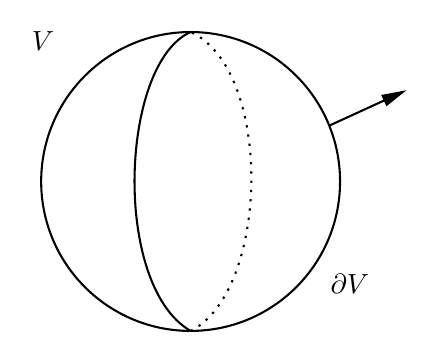
\begin{tikzpicture}[x=0.75pt,y=0.75pt,yscale=-1,xscale=1]
        %uncomment if require: \path (0,202); %set diagram left start at 0, and has height of 202

        %Shape: Circle [id:dp4776865069078362] 
        \draw   (181,103) .. controls (181,63.24) and (213.24,31) .. (253,31) .. controls (292.76,31) and (325,63.24) .. (325,103) .. controls (325,142.76) and (292.76,175) .. (253,175) .. controls (213.24,175) and (181,142.76) .. (181,103) -- cycle ;
        %Curve Lines [id:da18441231349656295] 
        \draw    (253,31) .. controls (219,46.06) and (215,153.06) .. (253,175) ;
        %Curve Lines [id:da32271069130490604] 
        \draw  [dash pattern={on 0.84pt off 2.51pt}]  (253,175) .. controls (291,156.06) and (293,49.06) .. (253,31) ;
        %Straight Lines [id:da8341320487347765] 
        \draw    (320,76) -- (355.18,59.89) ;
        \draw [shift={(357,59.06)}, rotate = 515.4] [fill={rgb, 255:red, 0; green, 0; blue, 0 }  ][line width=0.08]  [draw opacity=0] (12,-3) -- (0,0) -- (12,3) -- cycle    ;

        % Text Node
        \draw (175,29.4) node [anchor=north west][inner sep=0.75pt]    {$V$};
        % Text Node
        \draw (319,146.4) node [anchor=north west][inner sep=0.75pt]    {$\partial V$};
        % Text Node
        \draw (361,50.4) node [anchor=north west][inner sep=0.75pt]    {$\nuu$};

    \end{tikzpicture}
\end{figure}
\FloatBarrier

\begin{enumerate}
    \item $e=e(x,t)$ è l'energia interna per unità di massa, di conseguenza il tasso di variazione è descritto da
          \begin{equation*}
              \frac{\de}{\dt}\int _{V} e\rho \dxx
          \end{equation*}
    \item La sorgente esterna è descritta da
          \begin{equation*}
              \int _{V} r\rho \dxx
          \end{equation*}
    \item Il flusso attraverso $\partial V$ lo descriviamo tramite un vettore flusso di calore $\mathbf{q}$, che misura il calore per unità di area. Consideriamo anche $\displaystyle \nuu$ versore normale \emph{uscente}, allora dal momento che la componente tangente non comporta una variazione di calore nel corpo, il flusso entrante è dato da
          \begin{equation*}
              -\int _{\partial V}\mathbf{q} \cdotp \nuu \dsig
          \end{equation*}
\end{enumerate}

Mettendo insieme
\begin{equation*}
    \frac{\de}{\dt}\int _{V} e\rho \dxx=\int _{V} r\rho \dxx-\int _{\partial V}\mathbf{q} \cdotp \nuu \dsig
\end{equation*}
Supponendo di poter portare la derivata dentro l'integrale e applicando il teorema della divergenza
\begin{equation*}
    \int _{V} e_{t} \rho \dxx=\int _{V} r\rho \dxx-\int _{V}\mathrm{div}\mathbf{q} \dxx
\end{equation*}
Per l'arbitrarietà di $V$ deduciamo la \textbf{legge fondamentale della conduzione del calore}
\begin{equation*}
    \boxed{e_{t} \rho =-\mathrm{div}\mathbf{q} +r\rho }
\end{equation*}

\LezioneS{1/3/2021}

Per ricavare l'\textbf{equazione del calore} occorrono delle leggi costitutive per le quantità $e$ e $\displaystyle \mathbf{q}$:
\begin{itemize}
    \item \textbf{Legge di Fourier} (proporzionalità lineare tra flusso e gradiente della temperatura):
          \begin{equation*}
              \mathbf{q} =-k\nabla \theta
          \end{equation*}dove $k >0$ è la conduttività termica (dipendente dal materiale), $\displaystyle \theta $ la temperatura (assoluta) e il segno meno indica che il flusso del calore avviene verso zone a temperatura minore.
    \item \textbf{Proporzionalità lineare tra energia interna e temperatura assoluta:}
          \begin{equation*}
              e=c_{v} \theta
          \end{equation*}
          dove $\displaystyle c_{v}$ è il calore specifico a volume costante
\end{itemize}
$k$ e $\displaystyle c_{v}$ sono costanti in condizioni standard, per cui li supporrò tali.

Sostituendo le relazioni costitutive nella \textbf{legge fondamentale della conduzione del calore} ottengo:
\begin{equation*}
    \boxed{\rho c_{v} \theta _{t} =k\Delta \theta \ +\ r\rho }
\end{equation*}
Da cui, dividendo per $\displaystyle \rho c_{v}$, deduco l'\textbf{equazione del calore} in dimensione $n$ generica:
\begin{equation*}
    D=\frac{k}{\rho c_{v}} \quad \text{coefficiente di diffusione,} \quad f=\frac{r}{c_{v}}, \qquad \boxed{\theta _{t} -D\Delta \theta =f}
\end{equation*}

\section{Problemi ben posti in dimensione spaziale \texorpdfstring{$n=1$}{n=1}}

Considero l'evoluzione temporale della temperatura in una sbarra cilindrica di sezione trasversale $A$ e lunghezza $L$. Sotto le ipotesi:
\begin{enumerate}
    \item  raggio $\ll$ lunghezza;
    \item  sbarra isolata termicamente lungo la superficie laterale.
\end{enumerate}

Posso assumere che il flusso di calore avvenga in una sola direzione (l'asse $x$):
\begin{equation*}
    q=-ku_{x}\mathbf{L} \
\end{equation*}
Sostituendo nella \textbf{legge fondamentale della conduzione del calore} su un volume di controllo del tipo $\displaystyle V=A\times (x,x+\Delta x)$ e assumendo $\displaystyle u=u(x,t),\ e=e(x,t),\ r=r(x,t)$ (ben approssimabili a funzioni dipendenti da una sola variabile spaziale), l'area $A$ si semplifica e ottengo
\begin{equation*}
    \int ^{x+\Delta x}_{x} c_{v} \rho u_{t} \dx=\int ^{x+\Delta x}_{x} ku_{xx} \dx+\int ^{x+\Delta x}_{x} r\rho \dx
\end{equation*}
Da cui l'\textbf{equazione del calore monodimensionale:}
\begin{equation*}
    \boxed{u_{t} -Du_{xx} =f} \ \ \ x\in (0,L),\ 0< t< T
\end{equation*}

\textbf{Condizioni al bordo per garantire la buona posizione:}
\begin{itemize}
    \item Condizione \textbf{iniziale} (o di Cauchy) a $t=0$: assegna il profilo iniziale di temperatura
          \begin{equation*}
              u(x,0) =g(x),\ 0\leqslant x\leqslant L
          \end{equation*}
    \item Condizione \textbf{agli estremi} $\displaystyle x=0,\ x=L$
          \begin{itemize}
              \item Condizioni di \textbf{Dirichlet} (temperatura agli estremi) per $t\in (0,T]$
                    \begin{align*}
                        u(0,t) =h_{1}(t) \\
                        u(L,t) =h_{2}(t)
                    \end{align*}
              \item Condizioni di \textbf{Neumann} (flusso entrante agli estremi) per $t\in (0,T]$
                    \begin{align*}
                        -ku_{x}(0,t) =h_{1}(t) \\
                        ku_{x}(L,t) =h_{2}(t)
                    \end{align*}
              \item Condizioni di \textbf{radiazione} o di Robin (in uno o due estremi)
                    \begin{equation*}
                        ku_{x}(L,t) =\gamma (U-u(L,t)),\ t\in (0,T]
                    \end{equation*}

                    dove $\displaystyle \gamma  >0$ è una costante di proporzionalità e $U$ è la temperatura ambiente. Ponendo $\displaystyle \alpha =\frac{\gamma }{k}  >0$ e $\displaystyle \beta =\frac{}{}\frac{\gamma U}{k}$ posso riscrivere la condizione:
                    \begin{equation*}
                        u_{x}(L,t) +\alpha u(L,t) =\beta,\ t\in (0,T]
                    \end{equation*}
              \item Condizioni \textbf{miste}
          \end{itemize}
\end{itemize}

\begin{nb}
    La soluzione è cercata per i punti nell'insieme $\displaystyle Q_{T} =(0,L) \times (0,T)$, aperto connesso. Nessuna condizione finale per $\displaystyle 0< x< L,\ t=T$ è assegnata: le condizioni assegnate sono unicamente sulla \textbf{frontiera parabolica} di $\displaystyle Q_{T}$, formata dai 3 segmenti in grassetto. A breve ne formalizzeremo la definizione.
    \begin{figure}[H]
        \centering

        \tikzset{every picture/.style={line width=0.75pt}} %set default line width to 0.75pt        

        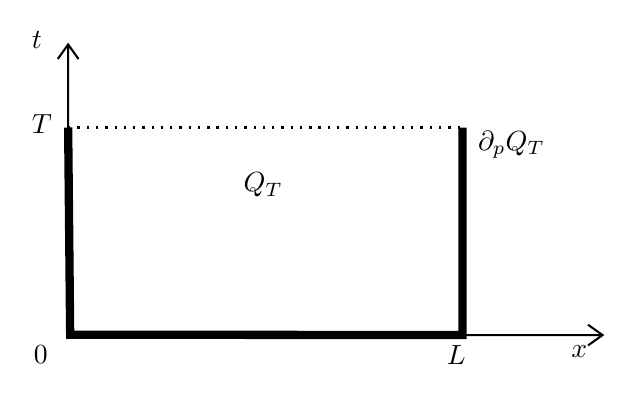
\begin{tikzpicture}[x=0.75pt,y=0.75pt,yscale=-1,xscale=1]
            %uncomment if require: \path (0,191); %set diagram left start at 0, and has height of 191

            %Shape: Axis 2D [id:dp16320631359033122] 
            \draw  (130,160) -- (387.47,160)(130,20) -- (130,160) -- cycle (380.47,155) -- (387.47,160) -- (380.47,165) (125,27) -- (130,20) -- (135,27)  ;
            %Straight Lines [id:da8618748502187668] 
            \draw [color={rgb, 255:red, 0; green, 0; blue, 0 }  ,draw opacity=1 ][line width=3]    (320,60) -- (320,160) -- (130.97,159.81) -- (130,60) ;
            %Straight Lines [id:da3361298498798142] 
            \draw [color={rgb, 255:red, 0; green, 0; blue, 0 }  ,draw opacity=1 ] [dash pattern={on 0.84pt off 2.51pt}]  (130,60) -- (320,60) ;

            % Text Node
            \draw (371,163.4) node [anchor=north west][inner sep=0.75pt]    {$x$};
            % Text Node
            \draw (111,12.4) node [anchor=north west][inner sep=0.75pt]    {$t$};
            % Text Node
            \draw (213,80.4) node [anchor=north west][inner sep=0.75pt]    {$Q_{T}$};
            % Text Node
            \draw (112,163.4) node [anchor=north west][inner sep=0.75pt]    {$0$};
            % Text Node
            \draw (311,163.4) node [anchor=north west][inner sep=0.75pt]    {$L$};
            % Text Node
            \draw (111,52.4) node [anchor=north west][inner sep=0.75pt]    {$T$};
            % Text Node
            \draw (326,60.4) node [anchor=north west][inner sep=0.75pt]    {$\partial _{p} Q_{T}$};

        \end{tikzpicture}
    \end{figure}
    \FloatBarrier
\end{nb}
In alcuni casi $x$ può variare in intervalli illimitati del tipo $\displaystyle (0,\infty)$ o $\displaystyle \mathbb{R}$ (sbarra ideale infinita). Il problema di Cauchy globale richiede allora delle condizioni aggiuntive che vedremo più avanti.
\begin{equation*}
    \begin{cases}
        u_{t} -Du_{xx} =f                       & x\in \mathbb{R},\ 0< t< T \\
        u(x,0) =g(x)                            & x\in \mathbb{R}           \\
        \text{condizioni\ } x\rightarrow \infty &
    \end{cases}
\end{equation*}

\section{Metodo di separazione delle variabili}

Esaminiamo un modello della sbarra in dimensione $n=1$. Sotto opportune ipotesi si può dimostrare facilmente che il problema è ben posto utilizzando il metodo di separazione delle variabili. Consideriamo il seguente problema di Cauchy-Dirichlet:
\begin{equation*}
    \begin{cases}
        u_{t} -Du_{xx} =0             & 0< x< L,\ t >0          \\
        u(x,0) =u_{0}                 & 0\leqslant x\leqslant L \\
        u(0,t) =u_{0},\ u(L,t) =u_{1} & t >0
    \end{cases}
\end{equation*}

Dove $\displaystyle u_{0},u_{1}$ costanti e $\displaystyle u_{1}  >u_{0}$. La sbarra è tenuta dunque inizialmente alla temperatura iniziale costante $\displaystyle u_{0}$. Successivamente, l'estremo $x=0$ mantiene la stessa temperatura (\textbf{estremo freddo}) mentre ho una discontinuità in $x=L$, mantenuto alla temperatura costante $\displaystyle u_{1}$(\textbf{estremo caldo}).

Attraverso un \textbf{ragionamento euristico} possiamo provare a capire come si evolverà la temperatura della sbarra nel tempo: dall'estremo caldo vi sarà un flusso entrante di calore che aumenterà la temperatura della sbarra, dall'estremo freddo un flusso uscente. All'inizio il flusso entrante sarà maggiore del flusso uscente ma, col passare del tempo (e con l'aumento della temperatura della sbarra), il flusso entrante diminuirà e il flusso uscente aumenterà fino a raggiungere una \textbf{situazione stazionaria} con i flussi bilanciati. Poiché siamo interessati al comportamento a regime, $t$ è illimitato.

\textbf{Variabili adimensionali}

Per motivi numerici e modellistici è utile riscrivere il problema di partenza utilizzando delle quantità \emph{indipendenti dalle unità di misura}, riscalando spazio, tempo e temperatura

\begin{itemize}
    \item \textbf{Spazio}: riscalo usando la lunghezza della sbarra $L$
          \begin{equation*}
              y=\frac{x}{L},\ 0< y< 1
          \end{equation*}
    \item \textbf{Tempo}: osserviamo che le dimensioni di $D$ sono
          \begin{equation*}
              [D] =\text{lunghezza}^{2} \times \text{tempo}^{-1}
          \end{equation*}
          Definisco
          \begin{equation*}
              \tau =\frac{L^{2}}{D},
          \end{equation*}
          che ha le dimensioni di un tempo e dipende dalle caratteristiche fisiche del problema. Riscalo il tempo usando la costante $\tau$
          \begin{equation*}
              s=\frac{t}{\tau}
          \end{equation*}
    \item \textbf{Temperatura}: definisco
          \begin{equation*}
              \vartheta (y,s) =\frac{u(Ly,\tau s) -u_{0}}{u_{1} -u_{0}}
          \end{equation*}
          osservo che
          \begin{align*}
              \vartheta (y,0) & =0, & \vartheta (1,s) & =1, \\
              \vartheta (0,s) & =0. &                 &
          \end{align*}
          inoltre
          \begin{equation*}
              \vartheta _{s} =\frac{u_{t} \tau }{u_{1} -u_{0}} ,\qquad \vartheta _{yy} =\frac{L^{2} u_{xx}}{u_{1} -u_{0}}
          \end{equation*}
          sostituendo $u_{t} =Du_{xx}$ e $\tau =L^{2} /D$ ottengo
          \begin{equation*}
              \vartheta _{s} =\frac{u_{t} \cdotp \tau }{u_{1} -u_{0}} =\frac{Du_{xx} \cdotp \frac{L^{2}}{D}}{u_{1} -u_{0}} =\frac{L^{2} u_{xx}}{u_{1} -u_{0}} =\vartheta _{yy} .
          \end{equation*}
\end{itemize}
quindi $\vartheta(y,s)$ soddisfa l'equazione del calore senza il termine $D$, normalizzato a 1. Posso riscrivere il mio problema in forma adimensionale.

\begin{equation*}
    \begin{cases}
        \vartheta_{s} -\vartheta_{yy} =0      & 0< y< 1,s >0 \\
        \vartheta(y,0) =0                     & 0< y< 1      \\
        \vartheta(0,s) =0,\ \vartheta(1,s) =1 & s >0
    \end{cases}
\end{equation*}

\begin{figure}[htpb]
    \centering


    \tikzset{every picture/.style={line width=0.75pt}} %set default line width to 0.75pt        

    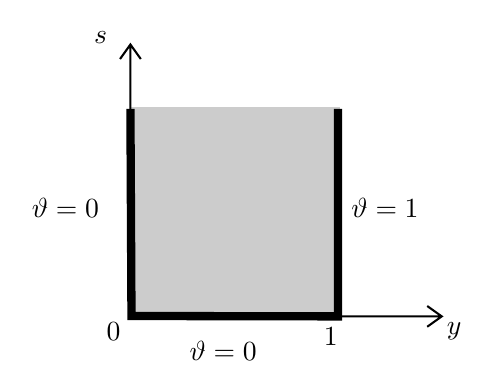
\begin{tikzpicture}[x=0.75pt,y=0.75pt,yscale=-1,xscale=1]
        %uncomment if require: \path (0,300); %set diagram left start at 0, and has height of 300

        %Shape: Square [id:dp9691905531249321] 
        \draw  [draw opacity=0][fill={rgb, 255:red, 0; green, 0; blue, 0 }  ,fill opacity=0.2 ] (150,90) -- (251,90) -- (251,191) -- (150,191) -- cycle ;
        %Shape: Axis 2D [id:dp1818781205642106] 
        \draw  (150,191) -- (300,191)(150,60) -- (150,191) -- cycle (293,186) -- (300,191) -- (293,196) (145,67) -- (150,60) -- (155,67)  ;
        %Straight Lines [id:da8052084024636774] 
        \draw [color={rgb, 255:red, 0; green, 0; blue, 0 }  ,draw opacity=1 ][line width=3]    (250,91) -- (250,191) -- (150.51,190.81) -- (150,91) ;

        % Text Node
        \draw (301,192.4) node [anchor=north west][inner sep=0.75pt]    {$y$};
        % Text Node
        \draw (131,52.4) node [anchor=north west][inner sep=0.75pt]    {$s$};
        % Text Node
        \draw (137,192.4) node [anchor=north west][inner sep=0.75pt]    {$0$};
        % Text Node
        \draw (241.67,195.07) node [anchor=north west][inner sep=0.75pt]    {$1$};
        % Text Node
        \draw (177,201.4) node [anchor=north west][inner sep=0.75pt]    {$\vartheta =0$};
        % Text Node
        \draw (255,132.4) node [anchor=north west][inner sep=0.75pt]    {$\vartheta =1$};
        % Text Node
        \draw (101,132.4) node [anchor=north west][inner sep=0.75pt]    {$\vartheta =0$};

    \end{tikzpicture}
\end{figure}
\FloatBarrier

\textbf{Condizioni omogenee}

Il problema in forma adimensionale presenta ancora una condizione non omogenea $\displaystyle \vartheta(1,s) =1$. Per usare il metodo di separazione delle variabili è necessario che tutto il sistema sia omogeneo.

Prendiamo in considerazione la soluzione stazionaria, per definizione essa non dipende dal tempo ($\vartheta^{st}(y)$) e si dimentica delle condizioni iniziali. Il sistema assume la forma

\begin{equation*}
    \begin{cases}
        \vartheta_{yy}^{st} =0            & 0< y< 1 \\
        \vartheta(0) =0,\ \vartheta(1) =1 &
    \end{cases}
\end{equation*}

Da cui integrando e imponendo le condizioni agli estremi si ricava

\begin{equation*}
    \vartheta^{st}(y) =y
\end{equation*}

\begin{nb}
    Ritornando alla forma dimensionale l'equazione stazionaria diventa
    \begin{align*}
        u^{st}(x) & =u_{0} +(u_{1} -u_{0})\vartheta^{st}(y) \\
                  & = u_{0} +(u_{1} -u_{0})y                \\
                  & = u_{0} +(u_{1} -u_{0}) \frac{x}{L}
    \end{align*}
    La soluzione stazionaria corrisponde dunque ad un flusso uniforme di calore lungo la sbarra del valore
    \begin{equation*}
        \text{flusso} = -k u^{st}_{x} = -\frac{k}{L}(u_{1} -u_{0})
    \end{equation*}
    \begin{figure}[H]
        \centering


        \tikzset{every picture/.style={line width=0.75pt}} %set default line width to 0.75pt        

        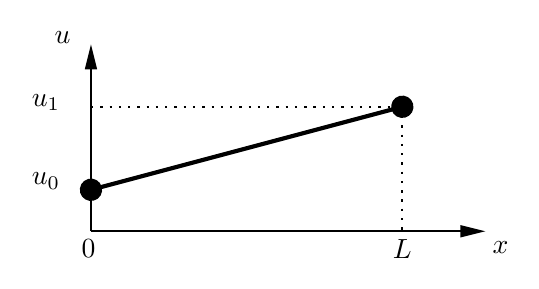
\begin{tikzpicture}[x=0.75pt,y=0.75pt,yscale=-1,xscale=1]
            %uncomment if require: \path (0,156); %set diagram left start at 0, and has height of 156

            %Straight Lines [id:da4473395182507709] 
            \draw    (160,110) -- (348,110) ;
            \draw [shift={(350,110)}, rotate = 180] [fill={rgb, 255:red, 0; green, 0; blue, 0 }  ][line width=0.08]  [draw opacity=0] (12,-3) -- (0,0) -- (12,3) -- cycle    ;
            %Straight Lines [id:da2693667751308695] 
            \draw [line width=1.5]    (160,90) -- (310,50) ;
            \draw [shift={(310,50)}, rotate = 345.07] [color={rgb, 255:red, 0; green, 0; blue, 0 }  ][fill={rgb, 255:red, 0; green, 0; blue, 0 }  ][line width=1.5]      (0, 0) circle [x radius= 4.36, y radius= 4.36]   ;
            \draw [shift={(160,90)}, rotate = 345.07] [color={rgb, 255:red, 0; green, 0; blue, 0 }  ][fill={rgb, 255:red, 0; green, 0; blue, 0 }  ][line width=1.5]      (0, 0) circle [x radius= 4.36, y radius= 4.36]   ;
            %Straight Lines [id:da6337447168637611] 
            \draw  [dash pattern={on 0.84pt off 2.51pt}]  (160,90) -- (160,110) ;
            %Straight Lines [id:da7853861441036836] 
            \draw  [dash pattern={on 0.84pt off 2.51pt}]  (310,50) -- (310,110) ;
            %Straight Lines [id:da4325323423726595] 
            \draw  [dash pattern={on 0.84pt off 2.51pt}]  (160,50) -- (310,50) ;
            %Straight Lines [id:da5448326316082119] 
            \draw    (160,110) -- (160,22) ;
            \draw [shift={(160,20)}, rotate = 450] [fill={rgb, 255:red, 0; green, 0; blue, 0 }  ][line width=0.08]  [draw opacity=0] (12,-3) -- (0,0) -- (12,3) -- cycle    ;

            % Text Node
            \draw (130,42.4) node [anchor=north west][inner sep=0.75pt]    {$u_{1}$};
            % Text Node
            \draw (130,80.4) node [anchor=north west][inner sep=0.75pt]    {$u_{0}$};
            % Text Node
            \draw (154,112.4) node [anchor=north west][inner sep=0.75pt]    {$0$};
            % Text Node
            \draw (304,112.4) node [anchor=north west][inner sep=0.75pt]    {$L$};
            % Text Node
            \draw (352,113.4) node [anchor=north west][inner sep=0.75pt]    {$x$};
            % Text Node
            \draw (141,12.4) node [anchor=north west][inner sep=0.75pt]    {$u$};

        \end{tikzpicture}
        \caption{Soluzione stazionaria $u^{st}(x)$.}
    \end{figure}
    \FloatBarrier
\end{nb}

Definendo a questo punto il \textbf{regime transitorio:}

\begin{equation*}
    U(y,s) =\vartheta^{st}(y) -\vartheta(y,s) =y-\vartheta(y,s)
\end{equation*}
esso tenderà a 0 per $\displaystyle s\rightarrow \infty $. $U$ soddisfa ancora l'equazione del calore e posso riscrivere il sistema con condizioni omogenee
\begin{equation*}
    \begin{cases}
        U_{s} -U_{yy} =0  & 0< y< 1,\ s >0          \\
        U(0,s) =U(1,s) =0 & s >0                    \\
        U(y,0) =y         & 0\leqslant y\leqslant 1
    \end{cases}
\end{equation*}
\textbf{Applicazione del metodo}

Ora che il problema è nella forma adatta voglio costruire una soluzione non banale mediante sovrapposizione di soluzioni particolari della forma

\begin{equation*}
    U(y,s) =w(s) v(y)
\end{equation*}

in modo tale che $\displaystyle v(0) =v(1) =0$

Sostituendo la forma della soluzione nell'equazione del calore ottengo

\begin{equation*}
    w'(s) v(y) -w(s) v'' (y) =0,\ \forall y\in (0,1),\ \forall s >0
\end{equation*}
Da cui dividendo per $\displaystyle w(s) v(y)$ e separando:
\begin{equation*}
    \frac{w'(s)}{w(s)} =\frac{v'' (y)}{v(y)} =\lambda
\end{equation*}
Dove $\displaystyle \lambda $ è una costante: infatti affinché l'identità tra i due rapporti sia valida per ogni $s >0$ ed ogni $\displaystyle y\in (0,1)$, essendo il primo membro funzione della sola variabile $s$ ed il secondo della sola variabile $y$, l'unica possibilità è che siano entrambi uguali ad una costante comune. Posso dividere il mio problema iniziale in due sottoproblemi
\begin{itemize}
    \item \textbf{Problema 1}
          \begin{equation*}
              \begin{cases}
                  v'' (y) -\lambda v(y) =0 \\
                  v(0) =v(1) =0
              \end{cases}
          \end{equation*}

          Si presentano 3 casi
          \begin{itemize}
              \item $\displaystyle \lambda  >0$, l'integrale generale è $\displaystyle v(y) =c_{1} e^{\sqrt{\lambda } y} +c_{2} e^{-\sqrt{\lambda } y}$, le condizioni al bordo
                    \begin{equation*}
                        \begin{cases}
                            v(0) =c_{1} +c_{2} =0 \\
                            v(1) =c_{1} e^{\sqrt{\lambda }} +c_{2} e^{-\sqrt{\lambda }} =0
                        \end{cases}
                    \end{equation*}da cui $\displaystyle c_{1} =c_{2} =0$, per cui otteniamo soluzioni banali e le scartiamo.
              \item $\displaystyle \lambda =0$, l'integrale generale è $\displaystyle v(y) =c_{1} y+c_{2}$, che unito alle condizioni al bordo dà $\displaystyle c_{1} =c_{2} =0$, soluzioni banali. Scartiamo anche queste.
              \item $\displaystyle \lambda =-\mu ^{2} < 0$, l'integrale generale è $\displaystyle v(y) =c_{1}\cos(\mu y) +c_{2}\sin(\mu y)$, le condizioni al bordo
                    \begin{equation*}
                        \begin{cases}
                            v(0) =c_{1} =0 \\
                            v(1) =\cancel{c_{1}\cos(\mu)} +c_{2}\sin(\mu) =c_{2}\sin(\mu) =0
                        \end{cases}
                    \end{equation*}

                    Escludendo le soluzioni banali ($\displaystyle c_{2} =0$) ottengo $\displaystyle \sin(\mu) =0$ e quindi $\displaystyle \mu =m\pi,\ m=1,2..$
          \end{itemize}

          Le soluzioni non banali del \textbf{problema 1} sono della forma\footnote{$\displaystyle v_{m}$ prendono il nome di autofunzioni e $\displaystyle \lambda _{m}$ di autovalori}
          \begin{equation*}
              \boxed{v_{m}(y) =c_{2}\sin(m\pi y),\ \lambda _{m} =-m^{2} \pi ^{2}}
          \end{equation*}

    \item \textbf{Problema 2}
          \begin{equation*}
              w'(s) =\lambda w(s)
          \end{equation*}

          Ha soluzioni non banali della forma
          \begin{equation*}
              \boxed{w_{m}(s) =Ce^{\lambda _{m} s} =Ce^{-m^{2} \pi ^{2} s}}
          \end{equation*}
\end{itemize}

Unendo le soluzioni dei due problemi ottengo infinite soluzioni numerabili
\begin{equation*}
    U_{m}(y,s) =A_{m} e^{-m^{2} \pi ^{2} s}\sin(m\pi y) \ \ \ \ m=1,2,\dotsc
\end{equation*}
\LezioneS{2/3/2021}

Nessuna di queste infinite soluzioni soddisfa la condizione iniziale $U(y,0) =y$, cerchiamo quindi di ottenere ciò che vogliamo sovrapponendo le infinite soluzioni
\begin{equation*}
    \boxed{U(y,s) =\sum\limits ^{\infty }_{m=1} A_{m} e^{-m^{2} \pi ^{2} s}\sin(m\pi y)}
\end{equation*}
Imponiamo la condizione iniziale, per farlo risulta
\begin{equation}
    U(y,s=0) =\sum\limits ^{\infty }_{m=1} A_{m}\sin(m\pi y) =y
    \label{eq:diff-cond-iniziale}
\end{equation}
quell'uguaglianza ad $y$ è da intendersi nel senso $L^{2}$, nello specifico dobbiamo sviluppare la funzione $f(y) =y$ in serie di Fourier nell'intervallo $(0,1)$ per calcolare i coefficienti $A_{m}$ che garantiscono la condizione iniziale.

Considerando una generica funzione $T$-periodica, si scrive in \textbf{serie di Fourier}\footnote{Il simbolo $\sim $ indica che l'uguaglianza vale nel senso $L^{2}\left(-\frac{T}{2},\frac{T}{2}\right)$. Indicando con $S_{N}(y)$ le somme parziali della serie, vale
    \begin{equation*}
        \lim _{N\rightarrow \infty }\int ^{T/2}_{-T/2}[ f(y) -S_{N}(y)]^{2} \dy=0
    \end{equation*}}
\begin{equation*}
    f(y) \sim \frac{a_{0}}{2} +\sum\limits ^{\infty }_{m=1}\left[ a_{m}\cos\left(\frac{2\pi m}{T} y\right) +b_{m}\sin\left(\frac{2\pi m}{T} y\right)\right]
\end{equation*}
i cui coefficienti sono, per $m\geqslant 0$
\begin{equation*}
    a_{m} =\frac{2}{T}\int ^{T/2}_{-T/2} f(y)\cos\left(\frac{2\pi m}{T} y\right) \dy\ \ \ \ b_{m} =\frac{2}{T}\int ^{T/2}_{-T/2} f(y)\sin\left(\frac{2\pi m}{T} y\right) \dy
\end{equation*}
Ricordiamo l'\textbf{identità di Parseval}
\begin{equation*}
    \frac{1}{T}\int ^{T/2}_{-T/2}[ f(y)]^{2} \dy=\frac{a^{2}_{0}}{2} +\sum\limits ^{\infty }_{m=1}\left(a^{2}_{m} +b^{2}_{m}\right)
\end{equation*}
Nel nostro caso vogliamo sviluppare la funzione $2$-periodica
\begin{equation*}
    f:[ -1,1]\rightarrow \mathbb{R} \ \ f(y) =y
\end{equation*}
È dispari, quindi è composta da soli seni, ovvero $a_{m}=0$ per ogni $m$.
\begin{align*}
    b_{m} & = \frac{2}{1-(-1)}\int ^{1}_{-1} y\sin(m\pi y) \dy \overset{\text{pari}}{=}2\int ^{1}_{0} y\sin(m\pi y) \dy               \\
          & \overset{\text{ipp}}{=}\left[ -\frac{2}{m\pi } y\cos(m\pi y)\right]^{1}_{0} +\frac{2}{m\pi }\int ^{1}_{0}\cos(m\pi y) \dy \\
          & =-2\frac{\cos(m\pi)}{m\pi } +\cancel{\frac{2}{m^{2} \pi ^{2}}[\sin(m\pi y)]^{1}_{0}} =\frac{2}{\pi }\frac{(-1)^{m+1}}{m}
\end{align*}
allora
\begin{equation}
    y\sim \sum\limits ^{\infty }_{m=1}\left[\frac{2}{\pi }\frac{(-1)^{m+1}}{m}\sin(m\pi y)\right]
    \label{eq:diff-y-fourier}
\end{equation}
Lo sviluppo è valido nell'intervallo $(-1,1)$, agli estremi è nulla, e converge uniformemente in ogni $[ a,b] \subset (-1,1)$.

La nostra soluzione \textit{candidata} è quindi, a seguito di \eqref{eq:diff-cond-iniziale} e \eqref{eq:diff-y-fourier} uguagliando i coefficienti
\begin{equation}
    A_{m} = \frac{2}{\pi }\frac{(-1)^{m+1}}{m} \qquad \boxed{U(y,s) =\sum\limits ^{\infty }_{m=1}\frac{2}{\pi }\frac{(-1)^{m+1}}{m}\sin(m\pi y) e^{-m^{2} \pi ^{2} s}}
    \label{eq:diff-candidata}
\end{equation}
\textbf{Questioni aperte}
\begin{itemize}
    \item \textbf{Q1} \textit{Condizione iniziale.} In che senso
          \begin{equation*}
              U(y,s)\rightarrow y\ \text{per} \ s\rightarrow 0^{+}
          \end{equation*}
    \item \textbf{Q2} Le $U_{m}$ sono tutte soluzioni dell'equazione del calore. Anche $U$ lo sarà? Se possiamo scambiare derivata e serie allora sì
          \begin{equation*}
              (\partial _{s} -\partial _{yy}) U(y,s)\overset{?}{=}\sum ^{\infty }_{m=1}(\partial _{s} -\partial _{yy}) U_{m} (y,s)=0
          \end{equation*}
    \item \textbf{Q3} $U$ soddisfa la \textit{condizione al bordo}?
          \begin{gather*}
              \lim\limits _{(y,s)\rightarrow (0,s_{0})} U(y,s) =0\\
              \lim\limits _{(y,s)\rightarrow (1,s_{0})} U(y,s) =0
          \end{gather*}
    \item \textbf{Q4} \textit{Unicità.}
    \item \textbf{Q5} È vero che $U(y,s)\rightarrow 0$ se $s\rightarrow \infty $?
\end{itemize}

\textbf{Risposte}
\begin{itemize}
\item \textbf{Q1} Consideriamo \eqref{eq:diff-candidata} e \eqref{eq:diff-y-fourier}. Per Parseval
\begin{gather*}
    \int ^{1}_{0}[ U(y,s) -y]^{2} \dy=\frac{2}{\pi ^{2}}\sum\limits ^{\infty }_{m=1}\frac{\left(e^{-m^{2} \pi ^{2} s} -1\right)^{2}}{m^{2}}\\
    \Rightarrow \ \ \frac{\left(e^{-m^{2} \pi ^{2} s} -1\right)^{2}}{m^{2}} \leqslant \frac{1}{m^{2}} \ \text{per} \ s\geqslant 0
\end{gather*}

Allora la serie converge uniformemente per il test di Weierstrass in $[ 0,+\infty)$ rispetto ad $s$, quindi
\begin{equation*}
    U(y,s) -y\rightarrow 0\ \text{in senso} \ L^{2}(0,1) \ \text{se} \ s\rightarrow 0
\end{equation*}
\item \textbf{Q2} Consideriamo \eqref{eq:diff-candidata}. Consideriamo una semistriscia del tipo
\begin{equation*}
    [ 0,1] \times [ s_{0},+\infty) \ \ s_{0}  >0
\end{equation*}

Il termine generale della serie $\sum U_{m}$ in modulo è maggiorato da
\begin{equation*}
    \left| \frac{(-1)^{m+1}}{m}\sin(m\pi y) e^{-m^{2} \pi ^{2} s}\right| \leqslant e^{-m^{2} \pi ^{2} s_{0}} \ \ \text{se} \ s >s_{0}
\end{equation*}

quindi per il test di Weierstrass la serie converge uniformemente.

Inoltre la serie delle derivate $\sum \partial _{s} U_{m},\sum \partial _{yy} U_{m}$ converge uniformemente sempre per il test di Weierstrass
\begin{gather*}
    \frac{\partial U_{m}}{\partial s} =\frac{\partial ^{2} U_{m}}{\partial y^{2}} =(-1)^{m+2} 2m\pi e^{-m^{2} \pi ^{2} s}\sin(m\pi y)\\
    \Rightarrow \ \ \left| \frac{\partial U_{m}}{\partial s}\right| =\left| \frac{\partial ^{2} U_{m}}{\partial y^{2}}\right| \leqslant 2m \pi e^{-m^{2} \pi ^{2} s_{0}},\ \ s\geqslant s_{0} \ \text{nella striscia}
\end{gather*}

Quindi possiamo scambiare serie e derivata e $U(y,s)$ è anch'essa soluzione.

Deduciamo anche che
\begin{equation*}
    U\in C^{\infty }([ 0,1] \times (0,+\infty))
\end{equation*}

avevamo una discontinuità nell'estremo destro, ma è diventata \textit{istantaneamente} regolare. Questo è l'\textbf{effetto regolarizzante} dell'equazione del calore.
\item \textbf{Q3} Sì perché la serie di $U$ è uniformemente convergente in $[ 0,1] \times [ s_{0},+\infty)$, $\forall s_{0}  >0$ e possiamo scambiare serie e limite.
\item \textbf{Q4} Usiamo il \textit{metodo dell'energia.}

Supponiamo che esistano due soluzioni nella stessa classe di $U$ con lo stesso dato iniziale $y$, assunto in senso $L^{2}(0,1)$. Poniamo
\begin{equation*}
    w=U-V
\end{equation*}

vogliamo mostrare che $w$ è nulla. La $w$ è soluzione dell'equazione con dati iniziali e al bordo nulli
\begin{equation*}
    \begin{cases}
        w_{s} -w_{yy} =0,  & \text{in} \ 0< y< 1,s >0     \\
        w(0,s) =w(1,s) =0, & \boxed{s >0}                 \\
        w(y,0) =0,         & \text{in senso} \ L^{2}(0,1)
    \end{cases}
\end{equation*}

Moltiplichiamo per $w$ da entrambi i lati e integriamo
\begin{gather*}
    \textcolor[rgb]{0.82,0.01,0.11}{\int ^{1}_{0}}\textcolor[rgb]{0.82,0.01,0.11}{ww}\textcolor[rgb]{0.82,0.01,0.11}{_{s}}\textcolor[rgb]{0.82,0.01,0.11}{\dy} =\textcolor[rgb]{0.29,0.56,0.89}{\int ^{1}_{0}}\textcolor[rgb]{0.29,0.56,0.89}{ww}\textcolor[rgb]{0.29,0.56,0.89}{_{yy}}\textcolor[rgb]{0.29,0.56,0.89}{\dy}\\
    \begin{aligned}
        \textcolor[rgb]{0.82,0.01,0.11}{\int ^{1}_{0}}\textcolor[rgb]{0.82,0.01,0.11}{ww}\textcolor[rgb]{0.82,0.01,0.11}{_{s}}\textcolor[rgb]{0.82,0.01,0.11}{\dy}  & =\frac{1}{2}\int ^{1}_{0}\frac{\partial }{\partial s} w^{2}(y,s) \dy=\frac{1}{2}\frac{\de}{\ds}\underbrace{\int ^{1}_{0} w^{2}(y,s) \dy}_{E(s)} =\frac{1}{2} E'(s) \\
        \textcolor[rgb]{0.29,0.56,0.89}{\int ^{1}_{0}}\textcolor[rgb]{0.29,0.56,0.89}{ww}\textcolor[rgb]{0.29,0.56,0.89}{_{yy}}\textcolor[rgb]{0.29,0.56,0.89}{\dy} & \overset{\text{ipp}}{=}\cancel{ww_{y} |^{1}_{0}} -\int ^{1}_{0}(w_{y})^{2} \dy\leqslant 0
    \end{aligned}
\end{gather*}

quindi $E(s)$ è non negativa, descrescente (non strettamente), inoltre $E(s)\rightarrow 0$ se $s\rightarrow 0$, allora
\begin{equation*}
    E(s) =0\ \ \forall s >0\ \ \Rightarrow \ \ \int ^{1}_{0} w^{2}(y,s) \dy=0\ \ \forall s >0
\end{equation*}

ma $w^{2}$ è continua per $s >0$ e non negativa. Non può essere che $w=0$ per $s >0$, ovvero $U=V$.
\item \textbf{Q5} Sempre per la convergenza uniforme della serie: se $\displaystyle s\geqslant 1$, il termine generale \begin{equation*}
    \left| \frac{(-1)^{m+1}}{m}\sin(m\pi y) e^{-m^{2} \pi ^{2} s}\right| \leqslant \frac{e^{-m^{2} \pi ^{2}}}{m}
\end{equation*}

quindi per il test di Weierstrass la serie converge uniformemente in $\displaystyle [ 0,1] \times [ 1,\infty)$, posso passare al limite sotto il segno di somma:
\begin{equation*}
    \lim_{s \to \infty} U(y,s) = \lim_{s \to \infty} \sum\limits ^{\infty }_{m=1}\cdots = \sum\limits ^{\infty }_{m=1} \lim_{s \to \infty} \cdots = 0
\end{equation*}
\end{itemize}

\textbf{Ritorno alle origini.}

Avevamo definito
\begin{equation*}
    \vartheta(y,s) =\frac{u(Ly,\tau s) -u_{0}}{u_{1} -u_{0}} \ \ \Rightarrow \ \ u(Ly,\tau s) =u_{0} +[ u_{1} -u_{0}] \vartheta(y,s)
\end{equation*}

e anche
\begin{equation*}
    \vartheta(y,s) =y-U(y,s) \ \ \ \ s=\frac{t}{\tau } \ \ \ \ y=\frac{x}{L} \ \ \ \ \tau =\frac{L^{2}}{D}
\end{equation*}
da cui possiamo finalmente riscrivere la soluzione nelle variabili originali
\begin{align*}
    u(x,t) & =u_{0} +[ u_{1} -u_{0}](y-U(y,s))                                                                                                                                                                                                                         \\
           & =u_{0} +[ u_{1} -u_{0}] y-[ u_{1} -u_{0}] U(y,s)                                                                                                                                                                                                          \\
           & =u_{0} +[ u_{1} -u_{0}]\frac{x}{L} -[ u_{1} -u_{0}]\sum\limits ^{\infty }_{m=1}\frac{2}{\pi }\frac{(-1)^{m+1}}{m} e^{-m^{2} \pi ^{2}\textcolor[rgb]{0.82,0.01,0.11}{\frac{D}{L^{2}}}\textcolor[rgb]{0.82,0.01,0.11}{t}}\sin\left(\frac{m\pi }{L} x\right)
\end{align*}
A regime notiamo che la supposizione iniziale era corretta, la temperatura si assesta a una soluzione stazionaria fatta come una retta
\begin{equation*}
    u(x,t) =u_{0} +[ u_{1} -u_{0}]\frac{x}{L} -\underbrace{[ u_{1} -u_{0}]\sum\limits ^{\infty }_{m=1}\frac{2}{\pi }\frac{(-1)^{m+1}}{m} e^{-m^{2} \pi ^{2}\frac{D}{L^{2}} t}\sin\left(\frac{m\pi }{L} x\right)}_{\rightarrow 0\ \text{per} \ t\rightarrow \infty }
\end{equation*}

\fg{0.7}{diffusione-soluzione-1d}

\section{Problemi in dimensione \texorpdfstring{$n>1$}{n>1}}

Sia $\displaystyle \Omega $ un dominio\footnote{ovvero un aperto connesso in $\displaystyle \mathbb{R}^{n}$.}. La temperatura sarà una $u=u(\x,t)$ che soddisfa $u_{t} -D\Delta u=f$ nel \textit{cilindro spazio-temporale}
\begin{equation*}
    Q_{T} =\Omega \times (0,T)
\end{equation*}

\fg{0.7}{diffusione-problema-2d}

Occorre assegnare
\begin{itemize}
    \item \textit{condizione iniziale}
          \begin{equation*}
              u(\x,0) =g(\x) \ \ \x \in \overline{\Omega }
          \end{equation*}
    \item \textit{condizioni sul bordo} $\partial \Omega $
          \begin{itemize}
              \item \textbf{Dirichlet}, si assegna la temperatura
                    \begin{equation*}
                        u(\sigg,t) =h(\sigg,t) \ \ \ \ \sigg \in \partial \Omega,t\in (0,T]
                    \end{equation*}
              \item \textbf{Neumann}, si assegna il flusso attraverso $\partial \Omega $. Indichiamo con $\nuu$ il versore normale al bordo in funzione del punto. Ricordiamo che $\partial _{\nuu} u=\nabla u\cdotp \nuu$. Si assegna
                    \begin{equation}
                        \partial _{\nuu}u(\sigg,t) =h(\sigg,t) \ \ \ \ \sigg \in \partial \Omega,t\in (0,T]
                    \end{equation}
              \item \textbf{Robin}, si assegna $(\alpha  >0)$
                    \begin{equation*}
                        \partial _{\nuu} u(\sigg,t) +\alpha u(\sigg,t) =\beta \ \ \ \ \sigg \in \partial \Omega,t\in (0,T]
                    \end{equation*}
          \end{itemize}
\end{itemize}

Le condizioni al bordo possono essere miste, per esempio $\partial \Omega =\gamma _{1} \cup \gamma _{2}$ e possiamo avere una condizione su $\gamma _{1}$ e una diversa condizione su $\gamma _{2}$.

Il problema è quindi determinare $u$ tale che
\begin{equation*}
    \begin{cases}
        u_{t} -D\Delta u=f            & \text{in} \ Q_{T}                        \\
        u(\x,0) =g(\x)                & \text{in} \ \overline{\Omega }           \\
        +\ \text{condizioni al bordo} & \text{su} \ \partial \Omega \times (0,T]
    \end{cases}
\end{equation*}
\textbf{Problema di Cauchy globale.}
\begin{equation*}
    \begin{cases}
        u_{t} -D\Delta u=f              & \x \in \mathbb{R}^{n},0< t< T \\
        u(\x,0) =g(\x)                  & \x \in \mathbb{R}^{n}         \\
        +\ \text{condizioni all'}\infty &
    \end{cases}
\end{equation*}
\begin{definition}
    [Frontiera parabolica] Le condizioni sono assegnate sulla frontiera parabolica del cilindro, cioè l'unione della base e della parte laterale $S_{T} =\partial \Omega \times (0,T]$
    \begin{equation*}
        \partial _{p} Q_{T} =(\overline{\Omega } \times \{t=0\}) \cup S_{T}
    \end{equation*}
\end{definition}
\section{Principi di massimo}

Il calore fluisce verso regioni dove la temperatura è più bassa, da ciò segue che la soluzione omogenea assume massimi e minimi globali sulla frontiera parabolica. Inoltre, risente di una irreversibilità temporale, il futuro non influenza il passato.

Indichiamo con $C^{2,1}(Q_{T})$ l'insieme delle funzioni di classe
\begin{equation*}
    \begin{array}{ l l }
        C^{2} & \text{rispetto a} \ x \\
        C^{1} & \text{rispetto a} \ t
    \end{array}
\end{equation*}
\textit{su misura} per l'equazione del calore.
\begin{theorem}
    [Principio di massimo (risp. minimo) debole] Sia $Q_{T} =\Omega \times (0,T)$, $\Omega $ dominio limitato. Sia $u\in C^{2,1}(Q_{T}) \cap C(\overline{Q}_{T})$ tale che
    \begin{equation*}
        u_{t} -D\Delta u=q\leqslant 0\ \ \text{in} \ Q_{T} \ \ \left(\text{risp.} \ \geqslant 0\right)
    \end{equation*}
    Allora il massimo (risp. minimo) di $u$ è assunto sulla frontiera parabolica di $Q_{T}$
    \begin{equation*}
        \max_{\overline{Q}_{T}} u=\max_{\partial _{p} Q_{T}} u\ \ \ \ \left(\text{risp.} \ \min_{\overline{Q}_{T}} u=\min_{\partial _{p} Q_{T}} u\right)
    \end{equation*}
\end{theorem}
La dicitura \emph{debole} è dovuta al fatto che garantisce che il massimo viene certamente assunto sulla frontiera parabolica, ma non esclude che sia assunto anche dentro. Per questo, servirà il Massimo Forte.
\begin{dimostrazione}
    Sia $\varepsilon >0$, definiamo $w=u-\varepsilon t$, allora
    \begin{equation}
        w_{t} -D\Delta w=q-\varepsilon < 0
        \label{eq:max-deb-contr-1}
    \end{equation}

    \begin{figure}[H]
        \centering
        \tikzset{every picture/.style={line width=0.75pt}} %set default line width to 0.75pt        

        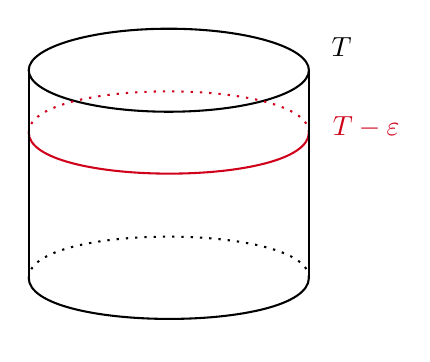
\begin{tikzpicture}[x=0.75pt,y=0.75pt,yscale=-1,xscale=1]
            %uncomment if require: \path (0,160); %set diagram left start at 0, and has height of 160

            %Shape: Ellipse [id:dp9954583197247324] 
            \draw   (163,30) .. controls (163,18.95) and (193.22,10) .. (230.5,10) .. controls (267.78,10) and (298,18.95) .. (298,30) .. controls (298,41.05) and (267.78,50) .. (230.5,50) .. controls (193.22,50) and (163,41.05) .. (163,30) -- cycle ;
            %Curve Lines [id:da36272626169586997] 
            \draw    (163,130) .. controls (163,156.25) and (297.8,156.6) .. (298,130) ;
            %Curve Lines [id:da5257514313993306] 
            \draw  [dash pattern={on 0.84pt off 2.51pt}]  (298,130) .. controls (298,103.75) and (163.2,103.4) .. (163,130) ;
            %Curve Lines [id:da6861700154443668] 
            \draw [color={rgb, 255:red, 208; green, 2; blue, 27 } ,draw opacity=1 ]   (163,60) .. controls (163,86.25) and (297.8,86.6) .. (298,60) ;
            %Curve Lines [id:da46362431718689145] 
            \draw [color={rgb, 255:red, 208; green, 2; blue, 27 } ,draw opacity=1 ] [dash pattern={on 0.84pt off 2.51pt}]  (298,60) .. controls (298,33.75) and (163.2,33.4) .. (163,60) ;
            %Straight Lines [id:da3476763854948828] 
            \draw    (163,30) -- (163,130) ;
            %Straight Lines [id:da7597497497420163] 
            \draw    (298,30) -- (298,130) ;

            % Text Node
            \draw (307.5,12.9) node [anchor=north west][inner sep=0.75pt]    {$T$};
            % Text Node
            \draw (308,50.9) node [anchor=north west][inner sep=0.75pt]  [color={rgb, 255:red, 208; green, 2; blue, 27 } ,opacity=1 ]  {$T-\varepsilon $};

        \end{tikzpicture}

    \end{figure}
    \FloatBarrier

    Supponiamo che esista un punto $(x_{0},t_{0}) \in \overline{Q}_{T-\varepsilon } \setminus \partial _{p} Q_{T-\varepsilon }$ punto di massimo per $w$, tale punto può trovarsi o all'interno o sul tappo superiore. Quindi, per definizione stessa di massimo:
    \begin{equation*}
        \begin{array}{ l l l }
            \text{all'interno} & w_{t} =0          & \Delta w\leqslant 0 \\
            \text{sul tappo}   & w_{t} \geqslant 0 & \Delta w\leqslant 0
        \end{array}
    \end{equation*}
    sul tappo è $w_{t}\geq 0$ perché potrebbe star crescendo ancora. Tuttavia in entrambi i casi
    \begin{equation}
        w_{t} -D\Delta w\geqslant 0
        \label{eq:max-deb-contr-2}
    \end{equation}
    le \eqref{eq:max-deb-contr-1} e \eqref{eq:max-deb-contr-2} sono in contraddizione, quindi il massimo sta sulla frontiera parabolica:
    \begin{equation*}
        \max_{\overline{Q}_{T-\varepsilon }} w=\max_{\partial _{p} Q_{T-\varepsilon }} w
    \end{equation*}

    Inoltre $w\leqslant u$ e $u=w+\varepsilon t\leqslant w+\varepsilon T$
    \begin{align*}
        \max_{\overline{Q}_{T-\varepsilon }} u & \leqslant \max_{\overline{Q}_{T-\varepsilon }} w+\varepsilon T    \\
                                               & =\max_{\partial _{p} Q_{T-\varepsilon }} w+\varepsilon T          \\
                                               & \leqslant \max_{\partial _{p} Q_{T-\varepsilon }} u+\varepsilon T
    \end{align*}
    Facendo tendere $\varepsilon \rightarrow 0$
    \begin{equation*}
        \max_{\overline{Q}_{T}} u\leqslant \max_{\partial _{p} Q_{T}} u
    \end{equation*}
    d'altro canto, essendo l'insieme a destra compreso in quello di sinistra, il massimo di sinistra deve essere almeno tanto quanto quello di destra
    \begin{equation*}
        \max_{\overline{Q}_{T}} u\geqslant \max_{\partial _{p} Q_{T}} u
    \end{equation*}
    da cui la tesi.
\end{dimostrazione}
\LezioneS{8/3/2021}
\section{Conseguenze del principio di massimo debole}

Sia $u\in C^{2,1}(Q_{T}) \cap C(\overline{Q}_{T})$ soluzione di
\begin{equation*}
    u_{t} -D\Delta u=0\ \ \text{in} \ Q_{T}
\end{equation*}
allora
\begin{equation*}
    \min_{\partial _{p} Q_{T}} u\leqslant \min_{\overline{Q}_{T}} u\leqslant \max_{\overline{Q}_{T}} u\leqslant \max_{\partial _{p} Q_{T}} u
\end{equation*}
\subsection{Corollario del massimo debole}

Siano $f_{1},f_{2}$ funzioni limitate in $Q_{T}$ e $u,v$ soluzioni di
\begin{gather*}
    u_{t} -D\Delta u=f_{1}\\
    v_{t} -D\Delta v=f_{2}
\end{gather*}
Allora
\begin{enumerate}
    \item \textit{Confronto.} Se $f_{1} \leqslant f_{2}$ in $Q_{T}$ e $u\leqslant v$ su $\partial _{p} Q_{T}$ allora
          \begin{equation*}
              u\leqslant v\ \text{in tutto} \ Q_{T}
          \end{equation*}
    \item Vale la stima
          \begin{equation*}
              \max_{\overline{Q}_{T}}| u-v| \leqslant \max_{\partial _{p} Q_{T}}| u-v| +T\sup _{Q_{T}}| f_{1} -f_{2}|
          \end{equation*}

          È una stabilità in norma $L^{\infty }$
          \begin{equation*}
              \Vert u-v\Vert _{L^{\infty }(\overline{Q}_{T})} \leqslant \Vert u-v\Vert _{L^{\infty }(\partial _{p} Q_{T})} +T\Vert f_{1} -f_{2}\Vert _{L^{\infty }(Q_{T})}
              \label{diffusione-stima-stabilita}
          \end{equation*}

          Questo implica l'\textbf{unicità e la dipendenza continua dai dati per il problema di Cauchy-Dirichlet} in $C^{2,1}(Q_{T}) \cap C(\overline{Q}_{T})$. Se uguali dati sulla frontiera e stessa sorgente esogena, allora $u=v$, infatti sia $u$ soluzione di
          \begin{equation*}
              \begin{cases}
                  u_{t} -D\Delta u=f & \text{in} \ Q_{T}                                \\
                  u=h                & \text{su} \ S_{T}                                \\
                  u=g                & \text{per} \ t=0\ \text{in} \ \overline{\Omega }
              \end{cases}
          \end{equation*}se $v$ è un'altra soluzione allora $w=u-v$ soddisfa
          \begin{equation*}
              \begin{cases}
                  w_{t} -D\Delta w=0 & \text{in} \ Q_{T}                                \\
                  w=0                & \text{su} \ S_{T}                                \\
                  w=0                & \text{per} \ t=0\ \text{in} \ \overline{\Omega }
              \end{cases}
          \end{equation*}
          allora \eqref{diffusione-stima-stabilita} diventa
          \begin{equation*}
              \Vert w\Vert _{L^{\infty }(\overline{Q}_{T})} \leqslant 0+0\ \ \Rightarrow \ \ u=v.
          \end{equation*}
\end{enumerate}
\subsection{Principio di massimo forte}

Se prendiamo un problema del tipo

\begin{figure}[htpb]
    \centering
    \tikzset{every picture/.style={line width=0.75pt}} %set default line width to 0.75pt        

    \begin{tikzpicture}[x=0.75pt,y=0.75pt,yscale=-1,xscale=1]
        %uncomment if require: \path (0,297); %set diagram left start at 0, and has height of 297

        %Straight Lines [id:da3946008733456672] 
        \draw    (200,214.31) -- (508,214.31) ;
        \draw [shift={(510,214.31)}, rotate = 180] [fill={rgb, 255:red, 0; green, 0; blue, 0 }  ][line width=0.08]  [draw opacity=0] (12,-3) -- (0,0) -- (12,3) -- cycle    ;
        %Straight Lines [id:da3125287839949542] 
        \draw    (200,214.31) -- (200,20.31) ;
        \draw [shift={(200,18.31)}, rotate = 450] [fill={rgb, 255:red, 0; green, 0; blue, 0 }  ][line width=0.08]  [draw opacity=0] (12,-3) -- (0,0) -- (12,3) -- cycle    ;
        %Straight Lines [id:da35837250143803123] 
        \draw    (200,58.31) -- (370,58.31) ;
        %Straight Lines [id:da9781100684099335] 
        \draw    (200,118.31) -- (370,118.31) ;
        %Curve Lines [id:da007305458198421322] 
        \draw    (138,247.31) .. controls (142.9,210.07) and (163.17,180.52) .. (189.39,164.29) ;
        \draw [shift={(191,163.31)}, rotate = 509.35] [fill={rgb, 255:red, 0; green, 0; blue, 0 }  ][line width=0.08]  [draw opacity=0] (12,-3) -- (0,0) -- (12,3) -- cycle    ;
        %Curve Lines [id:da5491813976204125] 
        \draw    (183,265.31) .. controls (208.74,263.33) and (244.28,250.57) .. (280.89,225.09) ;
        \draw [shift={(282,224.31)}, rotate = 504.9] [fill={rgb, 255:red, 0; green, 0; blue, 0 }  ][line width=0.08]  [draw opacity=0] (12,-3) -- (0,0) -- (12,3) -- cycle    ;
        %Curve Lines [id:da8634803668913487] 
        \draw    (185,281.31) .. controls (377.04,309.17) and (475.02,248.92) .. (384.38,174.44) ;
        \draw [shift={(383,173.31)}, rotate = 398.88] [fill={rgb, 255:red, 0; green, 0; blue, 0 }  ][line width=0.08]  [draw opacity=0] (12,-3) -- (0,0) -- (12,3) -- cycle    ;
        %Straight Lines [id:da3716594049457218] 
        \draw    (370,214.31) -- (370,58.31) ;
        %Curve Lines [id:da18228789256355693] 
        \draw    (377.19,90.81) .. controls (394.92,86.66) and (417.92,78.71) .. (440,64.31) ;
        \draw [shift={(375,91.31)}, rotate = 347.47] [fill={rgb, 255:red, 0; green, 0; blue, 0 }  ][line width=0.08]  [draw opacity=0] (12,-3) -- (0,0) -- (12,3) -- cycle    ;
        %Curve Lines [id:da1615187343378126] 
        \draw    (182.81,87.81) .. controls (165.08,83.66) and (142.08,75.71) .. (120,61.31) ;
        \draw [shift={(185,88.31)}, rotate = 192.53] [fill={rgb, 255:red, 0; green, 0; blue, 0 }  ][line width=0.08]  [draw opacity=0] (12,-3) -- (0,0) -- (12,3) -- cycle    ;

        % Text Node
        \draw (184,5.4) node [anchor=north west][inner sep=0.75pt]    {$t$};
        % Text Node
        \draw (179,48.4) node [anchor=north west][inner sep=0.75pt]    {$T$};
        % Text Node
        \draw (179,105.4) node [anchor=north west][inner sep=0.75pt]    {$\frac{\pi }{2}$};
        % Text Node
        \draw (125,255.4) node [anchor=north west][inner sep=0.75pt]    {$u=1$};
        % Text Node
        \draw (512,217.71) node [anchor=north west][inner sep=0.75pt]    {$x$};
        % Text Node
        \draw (187,217.4) node [anchor=north west][inner sep=0.75pt]    {$0$};
        % Text Node
        \draw (372,217.71) node [anchor=north west][inner sep=0.75pt]    {$L$};
        % Text Node
        \draw (445,48.4) node [anchor=north west][inner sep=0.75pt]    {$u=\sin t$};
        % Text Node
        \draw (75,37.4) node [anchor=north west][inner sep=0.75pt]    {$u=\sin t$};
        % Text Node
        \draw (240,138.4) node [anchor=north west][inner sep=0.75pt]    {$u_{t} -u_{xx} =0$};
        % Text Node
        \draw (254,175.4) node [anchor=north west][inner sep=0.75pt]    {$\text{qui} \ u=1$};

    \end{tikzpicture}

\end{figure}
\FloatBarrier

$u=1$ per $0\leqslant t\leqslant \pi /2$

Il massimo di $u$ sulla frontiera parabolica è
\begin{equation*}
    \max_{\partial _{p} Q_{T}} u=1
\end{equation*}
e il massimo di $u$ su tutto è
\begin{equation*}
    \max_{\overline{Q}_{T}} u=1
\end{equation*}
Tuttavia nel rettangolo fino a che $t=\pi /2$ il massimo non è assunto solo sulla frontiera, ma anche tutto all'interno. Si dimostra che è l'unica possibilità affinché avvenga, ovvero che \textbf{il massimo può essere assunto all'interno solo se fino a quel punto }$u$\textbf{ è rimasto costante (Principio di Massimo Forte).}
\fg[Principio di massimo forte. Si può notare come una volta usciti dalla zona dove si assume il massimo, non viene più raggiunto nei tempi successivi.]{0.6}{fig-max-forte}

\section{Soluzione fondamentale \texorpdfstring{$n=1$}{n=1}}

In $x=0$ sia concentrata una sorgente di calore \textbf{istantanea.} Indichiamo con $u^{\star }$ la temperatura della sbarra, vogliamo determinare l'evoluzione di $u^{\star },t\geqslant 0$.

\begin{figure}[htpb]
    \centering
    \tikzset{every picture/.style={line width=0.75pt}} %set default line width to 0.75pt        

    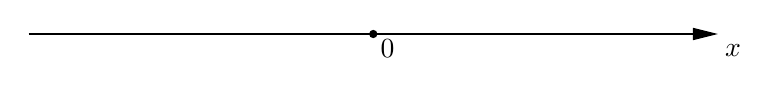
\begin{tikzpicture}[x=0.75pt,y=0.75pt,yscale=-1,xscale=1]
        %uncomment if require: \path (0,40); %set diagram left start at 0, and has height of 40

        %Straight Lines [id:da34140184544932506] 
        \draw    (130,13) -- (460,13) ;
        \draw [shift={(462,13)}, rotate = 180] [fill={rgb, 255:red, 0; green, 0; blue, 0 }  ][line width=0.08]  [draw opacity=0] (12,-3) -- (0,0) -- (12,3) -- cycle    ;
        %Shape: Circle [id:dp7601981243480558] 
        \draw  [draw opacity=0][fill={rgb, 255:red, 0; green, 0; blue, 0 } ,fill opacity=1 ] (294,13) .. controls (294,11.9) and (294.9,11) .. (296,11) .. controls (297.1,11) and (298,11.9) .. (298,13) .. controls (298,14.1) and (297.1,15) .. (296,15) .. controls (294.9,15) and (294,14.1) .. (294,13) -- cycle ;

        % Text Node
        \draw (464,16.4) node [anchor=north west][inner sep=0.75pt]    {$x$};
        % Text Node
        \draw (298,14.4) node [anchor=north west][inner sep=0.75pt]    {$0$};

    \end{tikzpicture}

\end{figure}
\FloatBarrier

Non ci sono sorgenti esogene $(f=0)$ quindi sicuramente soddisfa l'equazione del calore omogenea
\begin{equation*}
    u^{\star }_{t} -D u^{\star }_{xx} =0,\ \ x\in \mathbb{R},t >0
\end{equation*}
Vi è assenza di produzione o assorbimento di calore, allora l'energia si conserva
\begin{equation*}
    \int _{\mathbb{R}} \rho c_{v} u^{\star }(x,t) \dx=E\ \text{costante},\ \ t >0
\end{equation*}
Se scriviamo $Q=\frac{E}{\rho c_{v}}$ diventa
\begin{equation*}
    \int _{\mathbb{R}} u^{\star }(x,t) \dx=Q,\ \ t >0
\end{equation*}
La grandezza $Q$ ha le dimensioni di una temperatura per una lunghezza.

Inoltre $u^{\star }(x,t)$ è una funzione pari in $x$ e non negativa
\begin{equation*}
    u^{\star }(-x,t) =u^{\star }(x,t) \ \ \ \ \ \ \ \ u^{\star } \geqslant 0,\forall x\in \mathbb{R},\forall t >0
\end{equation*}
Per determinare $u^{\star }$ useremo $2$ passi
\subsection{Passo \texorpdfstring{$1$}{1}}

Dimostriamo che $u^{\star }$ è della forma
\begin{equation*}
    u^{\star }(x,t) =\frac{Q}{\sqrt{Dt}} \cdotp U\left(\frac{x}{\sqrt{Dt}}\right)
\end{equation*}
ponendo $\xi \in \mathbb{R}$, $U(\xi) \geqslant 0,\forall \xi $ la parità di $u^{\star }$ si riflette su $U$
\begin{equation*}
    U(\xi) =U(-\xi)
\end{equation*}
La cosa importante è che per questo primo passo non useremo l'equazione differenziale, ma useremo l'\textbf{analisi dimensionale}.
\begin{oss}
    [sull'Analisi Dimensionale] Supponiamo di essere in un sistema fisico, abbiamo una classe di sistemi di unità di misura, in riferimento ad alcune grandezze che riteniamo fondamentali. Per esempio \textit{lunghezza, massa e tempo} si possono misurare in
    \begin{equation*}
        \begin{array}{ c c c }
            L  & M  & T   \\
            m  & kg & sec \\
            cm & g  & sec
        \end{array}
    \end{equation*}
    Ad esempio
    \begin{equation*}
        [ \rho ] =L^{-3} M^{1} T^{0}
    \end{equation*}
    possiamo associare a tale scrittura un vettore le cui componenti sono gli esponenti
    \begin{equation*}
        \begin{pmatrix}
            L \\
            M \\
            T
        \end{pmatrix} \leftrightarrow \begin{pmatrix}
            -3 \\
            1  \\
            0
        \end{pmatrix}
    \end{equation*}
\end{oss}
L'analisi dimensionale è basata sul seguente teorema.
\begin{theorem}
    [Pi di Buckingham] Sia
    \begin{equation}
        q=f(q_{1},\dotsc,q_{n}) \tag{R}
        \label{eq:teo-pi-buckingham}
    \end{equation}
    una relazione \textbf{completa} (invariante al cambio di sistema di unità di misura nell'ambito di una stessa classe).

    Sia $1\leqslant k\leqslant n$ il massimo numero di grandezze dimensionalmente indipendenti tra le $q_{1},\dotsc,q_{n}$\footnote{poi si vedrà come determinare quali sono, ci avvarremo dell'algebra lineare.}. Siano per esempio le prime $q_{1},\dotsc,q_{k}$ (si dicono \textbf{quantità primarie}).

    Allora \eqref{eq:teo-pi-buckingham} si può scrivere nella forma
    \begin{equation*}
        \Pi =\mathcal{F}(\Pi _{1},\dotsc,\Pi _{n-k})
    \end{equation*}
    dove $\Pi _{1},\dotsc,\Pi _{n-k}$ sono \textbf{adimensionali}, ovvero numericamente non cambiano in qualunque modi si scali il sistema o le unità di misura (il vettore è nullo), espresse in termini di $q_{1},\dotsc,q_{n}$.
\end{theorem}
Applichiamo il tutto alla nostra situazione. Le grandezze fondamentali sono $\Theta,L,T$.
\begin{equation*}
    u^{\star } =f(x,t,D,Q) \ \ \ \ n=4
\end{equation*}
Abbiamo
\begin{equation*}
    \begin{array}{ l l }
        (x) =\Theta ^{0} L^{1} T^{0}  & \leftrightarrow \ \ \begin{pmatrix}
            0 \\
            1 \\
            0
        \end{pmatrix} \\\\
        (t) =\Theta ^{0} L^{0} T^{1}  & \leftrightarrow \ \ \begin{pmatrix}
            0 \\
            0 \\
            1
        \end{pmatrix} \\\\
        (D) =\Theta ^{0} L^{2} T^{-1} & \leftrightarrow \ \ \begin{pmatrix}
            0 \\
            2 \\
            -1
        \end{pmatrix} \\\\
        (Q) =\Theta ^{1} L^{1} T^{0}  & \leftrightarrow \ \ \begin{pmatrix}
            1 \\
            1 \\
            0
        \end{pmatrix}
    \end{array}
\end{equation*}
$t,D,Q$ sono linearmente indipendenti, di conseguenza li scegliamo come grandezze primarie. Esprimiamo le dimensioni delle grandezze secondarie in termini di quelle delle primarie
\begin{itemize}
    \item Per la $x$

          \begin{equation*}
              [ x] \leftrightarrow \begin{pmatrix}
                  0 \\
                  1 \\
                  0
              \end{pmatrix} =\alpha \begin{pmatrix}
                  0 \\
                  0 \\
                  1
              \end{pmatrix} +\beta \begin{pmatrix}
                  0 \\
                  2 \\
                  -1
              \end{pmatrix} +\gamma \begin{pmatrix}
                  1 \\
                  1 \\
                  0
              \end{pmatrix} \ \ \ \ \gamma =0,\beta =\frac{1}{2},\alpha =\frac{1}{2}
          \end{equation*}

          Questo vuol dire che

          \begin{equation*}
              [ x] =[ t]^{1/2}[ D]^{1/2}[ Q]^{0}
          \end{equation*}

          ma quindi $\frac{x}{\sqrt{Dt}} =\Pi _{1}$ è adimensionale.
    \item Per la $u^{\star }$

          \begin{equation*}
              \left[ u^{\star }\right] \leftrightarrow \begin{pmatrix}
                  1 \\
                  0 \\
                  0
              \end{pmatrix} =\alpha \begin{pmatrix}
                  0 \\
                  0 \\
                  1
              \end{pmatrix} +\beta \begin{pmatrix}
                  0 \\
                  2 \\
                  -1
              \end{pmatrix} +\gamma \begin{pmatrix}
                  1 \\
                  1 \\
                  0
              \end{pmatrix} \ \ \ \ \gamma =1,\alpha =\beta =-\frac{1}{2}
          \end{equation*}

          Questo vuol dire che
          \begin{equation*}
              \left[ u^{\star }\right] =[ t]^{-1/2}[ D]^{-1/2}[ Q]^{1}
          \end{equation*}

          ma quindi $\frac{u^{\star }}{\frac{Q}{\sqrt{Dt}}} =\Pi $ è adimensionale
\end{itemize}

Riscriviamo ciò che abbiamo
\begin{equation*}
    \Pi \frac{Q}{\sqrt{Dt}} =f\left(\Pi _{1}\sqrt{Dt},t,D,Q\right) \ \ \Rightarrow \ \ \Pi =\frac{\sqrt{Dt}}{Q} f\left(\Pi _{1}\sqrt{Dt},t,D,Q\right)
\end{equation*}
che è della forma
\begin{equation*}
    \Pi =U(\Pi _{1},t,D,Q)
\end{equation*}
\textbf{Punto cruciale.} Anche $U$ deve essere adimensionale, ma se io cambio $t,D,Q$ cambiano numericamente le grandezze, per cui \textbf{non può dipender}e da $t,D,Q$.
\begin{equation*}
    \Rightarrow \ \ \Pi =U(\Pi _{1})
\end{equation*}
Torniamo alle variabili originali
\begin{equation*}
    \frac{u^{\star }}{\frac{Q}{\sqrt{Dt}}} =U\left(\frac{x}{\sqrt{Dt}}\right) \ \ \Rightarrow \ \ u^{\star } =\frac{Q}{\sqrt{Dt}} U\left(\frac{x}{\sqrt{Dt}}\right)
\end{equation*}
\subsection{Passo \texorpdfstring{$2$}{2}}

Dimostriamo che
\begin{equation*}
    U(\xi) =\frac{1}{\sqrt{4\pi }} e^{-\frac{\xi ^{2}}{4}}
\end{equation*}
Dobbiamo usare l'equazione del calore imponendo che $u^{\star }$ sia soluzione, poniamo $\xi =\frac{x}{\sqrt{Dt}}$, allora
\begin{align*}
    u^{\star }_{t}  & =\frac{Q}{\sqrt{D}}\left[ -\frac{1}{2} t^{-3/2} U(\xi) +t^{-1/2} U'(\xi)\frac{x}{\sqrt{D}}\left(-\frac{1}{2}\right) t^{-3/2}\right] \\
                    & =-\frac{Q}{\sqrt{D}}\frac{1}{2} t^{-3/2}[ U(\xi) +U'(\xi) \xi ]                                                                     \\
                    &                                                                                                                                     \\
    u^{\star }_{x}  & =\frac{Q}{\sqrt{Dt}} U'(\xi) \cdotp \frac{1}{\sqrt{Dt}} =\frac{Q}{Dt} U'(\xi)                                                       \\
                    &                                                                                                                                     \\
    u^{\star }_{xx} & =\frac{Q}{Dt} U''(\xi) \cdotp \frac{1}{\sqrt{Dt}} =\frac{Q}{\sqrt{D}} t^{-3/2}\frac{1}{D} U''(\xi)
\end{align*}
Sostituiamo nell'equazione del calore omogenea
\begin{gather*}
    u^{\star }_{t} -Du^{\star }_{xx} =\frac{Q}{\sqrt{D}} t^{-3/2}\left[ -\frac{1}{2} U(\xi) -\frac{1}{2} U'(\xi) \xi -U''(\xi)\right] =0\\
    \Rightarrow \ \ U''(\xi) +\frac{1}{2} \xi U'(\xi) +\frac{1}{2} U(\xi) =0
\end{gather*}
Tale termine può essere visto come una derivata
\begin{equation*}
    \frac{\de}{\dxi }\left[ U'(\xi) +\frac{1}{2} \xi U(\xi)\right] =0\ \ \Rightarrow \ \ U'(\xi) +\frac{1}{2} \xi U(\xi) =\text{costante}
\end{equation*}
Ma sappiamo che $U$ è pari e regolare in un certo senso, allora $U'(0) =0$. Imponendo quindi $\xi =0$ scopriamo che anche la costante è nulla. Abbiamo dunque
\begin{equation*}
    U'(\xi) +\frac{1}{2} \xi U(\xi) =0
\end{equation*}
È un'equazione a variabili separabili
\begin{equation*}
    \frac{U'}{U} =-\frac{1}{2} \xi \ \ \Rightarrow \ \ \log U=-\frac{1}{4} \xi ^{2} +k\ \ \Rightarrow \ \ U=ce^{-\frac{1}{4} \xi ^{2}}
\end{equation*}
Cos'è $c$? Non abbiamo ancora usato la conservazione dell'energia
\begin{equation*}
    \int _{\mathbb{R}} u^{\star }(x,t) \dx=Q
\end{equation*}
che si riduce a
\begin{equation*}
    Q = \int _{\mathbb{R}}\frac{Q}{\sqrt{Dt}} U\left(\frac{x}{\sqrt{Dt}}\right) \dx=\left\{\xi=\frac{x}{\sqrt{Dt}}\right\} = Q\int _{\mathbb{R}} U(\xi) d\xi
\end{equation*}
Allora possiamo procedere a determinare $c$
\begin{equation*}
    \int _{\mathbb{R}} U(\xi) d\xi =1\ \ \Rightarrow \ \ c\int _{\mathbb{R}} e^{-\frac{1}{4} \xi ^{2}} d\xi =1\ \ \Rightarrow \ \ \begin{cases}
        \xi =2z \\
        d\xi =2dz
    \end{cases}
\end{equation*}
Ricordando l'integrale di Gauss
\begin{equation*}
    2c\underbrace{\int _{\mathbb{R}} e^{-z^{2}} dz}_{\sqrt{\pi }} =1\ \ \Rightarrow \ \ c=\frac{1}{\sqrt{4\pi }}
\end{equation*}
Infine
\begin{equation*}
    \boxed{u^{\star }(x,t) =\frac{Q}{\sqrt{4\pi Dt}} e^{-\frac{x^{2}}{4Dt}}}
\end{equation*}
Nel caso in cui $Q=1$ si ottiene la \textbf{soluzione fondamentale.}
\begin{equation*}
    \boxed{\Gamma _{D}(x,t) =\frac{1}{\sqrt{4\pi Dt}} e^{-\frac{x^{2}}{4Dt}}}
\end{equation*}
Che ricorda la densità di probabilità di una normale di media $\mu=0$ e varianza $\sigma ^2 =2Dt$.
\fg[Soluzione fondamentale con $D=1$. Si può notare il picco iniziale che viene poi smussato.]{0.6}{fig-soluzione-fondamentale-calore}

\textbf{Dimostrazione in due righe del Teorema di Pitagora.}\footnote{Ovvero: come sparare a una mosca con un cannone (cit. S. Salsa).}

\begin{figure}[htpb]
    \centering
    \tikzset{every picture/.style={line width=0.75pt}} %set default line width to 0.75pt        

    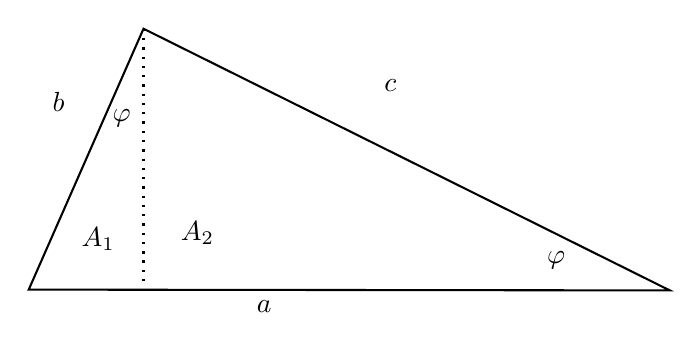
\begin{tikzpicture}[x=0.75pt,y=0.75pt,yscale=-1,xscale=1]
        %uncomment if require: \path (0,162); %set diagram left start at 0, and has height of 162

        %Shape: Right Triangle [id:dp542719595058683] 
        \draw   (150.8,133.44) -- (459.67,133.83) -- (206.11,7.74) -- cycle ;
        %Straight Lines [id:da8113900840921482] 
        \draw  [dash pattern={on 0.84pt off 2.51pt}]  (206.11,7.74) -- (206.11,132.68) ;

        % Text Node
        \draw (174.83,101.9) node [anchor=north west][inner sep=0.75pt]    {$A_{1}$};
        % Text Node
        \draw (222.67,99.19) node [anchor=north west][inner sep=0.75pt]    {$A_{2}$};
        % Text Node
        \draw (160.87,37.01) node [anchor=north west][inner sep=0.75pt]    {$b$};
        % Text Node
        \draw (320.64,30.69) node [anchor=north west][inner sep=0.75pt]    {$c$};
        % Text Node
        \draw (259.26,137.2) node [anchor=north west][inner sep=0.75pt]    {$a$};
        % Text Node
        \draw (399.12,113.73) node [anchor=north west][inner sep=0.75pt]    {$\varphi $};
        % Text Node
        \draw (189.71,45.13) node [anchor=north west][inner sep=0.75pt]    {$\varphi $};

    \end{tikzpicture}

\end{figure}
\FloatBarrier

\begin{equation*}
    A=A_{1} +A_{2} \ \ \ \ \begin{cases}
        A=\mathcal{F}(a,\varphi)      \\
        A_{1} =\mathcal{F}(b,\varphi) \\
        A_{2} =\mathcal{F}(c,\varphi)
    \end{cases} \ \ \ \ [ A] =L^{2}
\end{equation*}
Usiamo l'analisi dimensionale
\begin{equation*}
    \frac{A}{a^{2}} =\mathcal{F}^{\star }(\varphi) \ \text{adimensionale},\ \ \ \ A_{1} =b^{2}\mathcal{F}^{\star }(\varphi),\ \ \ \ A_{2} =c^{2}\mathcal{F}^{\star }(\varphi)
\end{equation*}
La funzione è la stessa perché i triangoli sono \emph{simili}. Quindi
\begin{gather*}
    a^{2}\mathcal{F}^{\star }(\varphi) =b^{2}\mathcal{F}^{\star }(\varphi) +c^{2}\mathcal{F}^{\star }(\varphi) \ \ \Rightarrow \ \ a^{2} =b^{2} +c^{2}\\
    \qed
\end{gather*}
\LezioneS{9/3/2021}
\subsection{Modellazione matematica della sorgente d'origine}

Per giungere alla soluzione fondamentale siamo partiti dall'evoluzione della temperatura causata da una sorgente istantanea e concentrata nell'origine. Qual è il modello matematico più adatto a descriverla?

Per la conservazione dell'energia
\begin{equation*}
    \int _{\mathbb{R}} \Gamma _{D}(x,t) =1,\ \forall t >0
\end{equation*}
Inoltre possiamo studiare il comportamento della soluzione fondamentale per $\displaystyle t\rightarrow 0^{+}$
\begin{equation*}
    \Gamma _{D}(x,t) =\frac{1}{\sqrt{4\pi Dt}} e^{-\frac{x^{2}}{4Dt}}\xrightarrow{t\rightarrow 0^{+}}
    \begin{cases}
        0,      & x\neq 0 \\
        \infty, & x=0
    \end{cases}
\end{equation*}
Nessuna funzione ha queste proprietà, ma si può modellare matematicamente la sorgente con una funzione generalizzata, una distribuzione: la \textbf{delta di Dirac }(nell'origine) $\displaystyle \delta _{0}$
\begin{equation*}
    ``\ \Gamma _{D}(x,0) =\delta _{0}(x) \ "
\end{equation*}
diventa la condizione iniziale.
\begin{definition}
    [delta di Dirac] Si chiama distribuzione di Dirac nell'origine la funzione generalizzata che si indica con $\displaystyle \delta _{0}$ e che agisce su una funzione test $\displaystyle \varphi $ nel seguente modo
    \begin{equation*}
        \int \delta (x) \varphi (x) \dx=\langle \delta,\varphi \rangle =\varphi (0)
    \end{equation*}
\end{definition}
Il limite che abbiamo fatto sopra è un limite nel senso delle distribuzioni, in $\displaystyle D'(\mathbb{R})$
\begin{equation*}
    \langle \Gamma _{D}(\cdotp,t),\varphi \rangle \xrightarrow{t\rightarrow 0^{+}} \langle \delta,\varphi \rangle =\varphi (0)
\end{equation*}
Se anziché nell'origine, la sorgente unitaria fosse concentrata in un punto $y$, dovrei modellarla con la distribuzione di Dirac in $y$, $\displaystyle \delta (x-y)$, e la funzione $\displaystyle \Gamma _{D}(x-y,t)$ è l'unica soluzione (grazie all'invarianza per traslazione spaziale) che soddisfi la condizione iniziale
\begin{equation*}
    ``\ \Gamma _{D}(x-y,0) =\delta (x-y)\ "
\end{equation*}
\subsection{Interpretazione della \texorpdfstring{$\displaystyle \Gamma _{D}(x,t)$}{soluzione}}
\begin{itemize}
    \item \textit{Unit source solution}: $\displaystyle \Gamma _{D}$ descrive la \textbf{concentrazione} di una sostanza nel punto $x$ al tempo $t$ generata dalla diffusione di una massa unitaria inizalmente concentrata nell'origine
    \item Altro punto di vista: sia una massa unitaria composta da un \textbf{numero }$N$\textbf{ di particelle}
          \begin{itemize}
              \item $\displaystyle \Gamma _{D}(x,t) \dx$ fornisce probabilità di trovare una particella in un intervallo del tipo $\displaystyle (x,x+\dx)$ al tempo $t$.
              \item $\displaystyle \Gamma _{D}(x,t) \dx$ fornisce la percentuale di particelle fra le $N$ che si trova in $\displaystyle (x,x+\dx)$ al tempo $t$.
          \end{itemize}
\end{itemize}
\begin{nb}
    Come già osservato in precedenza, per $t >0$ \ $\displaystyle \Gamma _{D}$ è $\displaystyle C^{\infty }(\mathbb{R} \times (0,+\infty))$. Si dimentica immediatamente della singolarità ed è positiva $\displaystyle \forall t >0$: la diffusione del calore è istantanea in tutta la sbarra.
\end{nb}
\subsection{Soluzione fondamentale in \texorpdfstring{$n>1$}{n>1}}

Con ragionamenti analoghi otteniamo
\begin{equation*}
    \Gamma _{D}(\x,t) =\frac{1}{(4\pi Dt)^{n/2}} e^{-\frac{| \x| ^{2}}{4Dt}}
\end{equation*}
e come condizione iniziale
\begin{gather*}
    ``\ \Gamma _{D}(\x,0) =\delta _{n}(\zer) \ "\\
    \int _{\mathbb{R}^{n}} \Gamma _{D}(\x,0) \varphi (\x) \dxx =\langle \delta _{n},\varphi \rangle =\varphi (\zer)
\end{gather*}
l'interpretazione della soluzione fondamentale è analoga e la conservazione dell'energia si esprime come
\begin{equation*}
    \int _{\mathbb{R}^{n}} \Gamma _{D}(\x,t) \dxx =1,\ \forall t >0
\end{equation*}
\section{Passeggiata aleatoria simmetrica (unidimensionale)}

Esploriamo ora la connesione tra modelli \textbf{deterministici} analizzati fin'ora e \textbf{probabilistici}. Vogliamo costruire modelli \textbf{continui} (nel nostro caso del tipo del moto browniano) come limite di modelli \textbf{discreti stocastici}.

Nel realizzare il procedimento si vede come l'equazione del calore possa essere approssimata con un'equazione alle differenze, risultato utile per alcuni metodi numerici che permettono il calcolo approssimato delle soluzioni.

Il nostro modello discreto, dato un passo spaziale di lunghezza $h$ e un intervallo temporale di durata $\displaystyle \tau $, prevede \textbf{una} particella di \textbf{massa unitaria} in moto lungo un asse (asse $x$) con le seguenti regole
\begin{enumerate}
    \item la particella si muove, in un tempo $\displaystyle \tau $, di $h$, partendo da $x=0$.
    \item la particella si muove verso destra o sinistra con probabilità $1/2$, in modo indipendente dai passi precedenti.
\end{enumerate}

La particella al tempo $\displaystyle t=N\tau $ (dopo $N$ passi) si troverà in
\begin{equation*}
    x=mh,\ m\in \mathbb{Z},\ -N\leqslant m\leqslant N
\end{equation*}
$x,m$ sono variabili aleatorie.

Voglio calcolare
\begin{equation*}
    p(x,t) =\text{probabilità di trovare la particella in} \ x\ \text{al tempo} \ t
\end{equation*}
Se $x=mh$ è la posizione della particella dopo $N$ passi, avrò fatto:
\begin{itemize}
    \item $k$ passi a destra ($k$ è una variabile aleatoria)
    \item $N-k$ passi a sinistra
\end{itemize}

con $\displaystyle 0\leqslant k\leqslant N$.
\begin{equation*}
    m=k-(N-k) =2k-N
\end{equation*}
dunque
\begin{align*}
    p(x,t) & =p_{k} =\frac{\text{\#cammini con} \ k\ \text{passi a destra}}{\text{\#cammini con} \ N\ \text{passi}} \\
           & =\frac{\binom{N}{k}}{2^{N}} =\binom{N}{k}\left(\frac{1}{2}\right)^{k}\left(1-\frac{1}{2}\right)^{N-k}
\end{align*}
$k$ ha legge binomiale di parametri $\displaystyle Bi\left(N,\frac{1}{2}\right)$.
\begin{itemize}
    \item valore atteso di $k$
          \begin{equation*}
              \mathbb{E}[k]=\langle k\rangle =Np=\frac{N}{2}
          \end{equation*}
    \item varianza di $k$
          \begin{equation*}
              \mathrm{Var}[k]=\langle k^{2} \rangle -\langle k\rangle ^{2} =np(1-p)=\frac{N}{4}
          \end{equation*}
    \item momento secondo di $k$
          \begin{equation*}
              \mathbb{E}[k^2]=\langle k^{2} \rangle =\frac{N}{4} +\langle k\rangle ^{2} =\frac{N+N^2}{4}
          \end{equation*}
\end{itemize}

Da cui si possono calcolare media e varianza di $x$:
\begin{itemize}
    \item media di $x$
          \begin{equation*}
              \langle x\rangle =h\langle m\rangle =h\langle 2k-N\rangle =h(2\langle k\rangle -N) =0
          \end{equation*}
    \item varianza di $x$
          \begin{align*}
              \mathrm{Var}[x]=\langle x^{2} \cancel{\rangle -\langle x \rangle^2} & =h^{2} \langle m^{2} \rangle =h^{2} \langle 4k^{2} -4Nk+N^{2} \rangle \\
                                                                                  & =h^{2}\left(4\langle k^{2} \rangle -4N\langle k\rangle +N^{2}\right)  \\
                                                                                  & =h^{2}\left(4 \frac{N+N^2}{4} -4 N \frac{N}{2} + N^2 \right)          \\
                                                                                  & =h^{2}\left(N^{2} +N-2N^{2} +N^{2}\right)                             \\
                                                                                  & =h^{2} N
          \end{align*}
\end{itemize}

Questi due valori sono \textbf{caratteristiche essenziali della passeggiata} da cui posso ricavare
\begin{equation*}
    \frac{\mathrm{Var[x]}}{t}=\frac{\langle x^{2} \rangle }{t} =\frac{h^{2} N}{\tau N} =\frac{h^{2}}{\tau }
\end{equation*}
prendendo la deviazione standard
\begin{equation*}
    d=\sqrt{\langle x^{2} \rangle } =\frac{h}{\sqrt{\tau }}\sqrt{t} \ \ \Rightarrow \ d\sim \sqrt{t}
\end{equation*}
questa relazione mi dice che le particelle diffondono dell'ordine della radice di $t$: in pratica, dopo $100$ secondi, mi sono mosso dell'ordine di $10$.

Per arrivare ad un modello continuo ora devo ricavare un'equazione alle differenze finite su cui fare un passaggio al limite per $\displaystyle h,\tau \rightarrow 0$ (mantenendo tuttavia le stesse caratteristiche della passeggiata: il rapporto $d,t$)

\begin{figure}[htpb]
    \centering

    \tikzset{every picture/.style={line width=0.75pt}} %set default line width to 0.75pt        

    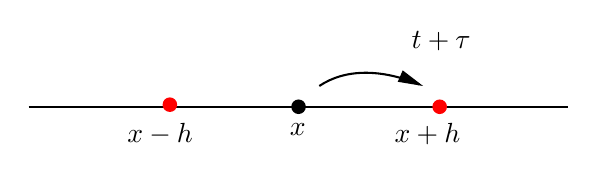
\begin{tikzpicture}[x=0.75pt,y=0.75pt,yscale=-1,xscale=1]
        %uncomment if require: \path (0,61); %set diagram left start at 0, and has height of 61

        %Straight Lines [id:da8969705158973058] 
        \draw [color={rgb, 255:red, 0; green, 0; blue, 0 }  ,draw opacity=1 ]   (120,30) -- (380,30) ;
        %Shape: Circle [id:dp7785723770796928] 
        \draw  [fill={rgb, 255:red, 0; green, 0; blue, 0 }  ,fill opacity=1 ] (247,30) .. controls (247,28.34) and (248.34,27) .. (250,27) .. controls (251.66,27) and (253,28.34) .. (253,30) .. controls (253,31.66) and (251.66,33) .. (250,33) .. controls (248.34,33) and (247,31.66) .. (247,30) -- cycle ;
        %Shape: Circle [id:dp7108075326392389] 
        \draw  [color={rgb, 255:red, 255; green, 0; blue, 0 }  ,draw opacity=1 ][fill={rgb, 255:red, 255; green, 0; blue, 0 }  ,fill opacity=1 ] (185,29) .. controls (185,27.34) and (186.34,26) .. (188,26) .. controls (189.66,26) and (191,27.34) .. (191,29) .. controls (191,30.66) and (189.66,32) .. (188,32) .. controls (186.34,32) and (185,30.66) .. (185,29) -- cycle ;
        %Shape: Circle [id:dp23106628962253284] 
        \draw  [color={rgb, 255:red, 255; green, 0; blue, 0 }  ,draw opacity=1 ][fill={rgb, 255:red, 255; green, 0; blue, 0 }  ,fill opacity=1 ] (315,30) .. controls (315,28.34) and (316.34,27) .. (318,27) .. controls (319.66,27) and (321,28.34) .. (321,30) .. controls (321,31.66) and (319.66,33) .. (318,33) .. controls (316.34,33) and (315,31.66) .. (315,30) -- cycle ;
        %Curve Lines [id:da263551245188425] 
        \draw    (260,20) .. controls (272.61,11.51) and (289.92,11.73) .. (308.29,19.28) ;
        \draw [shift={(310,20)}, rotate = 203.47] [fill={rgb, 255:red, 0; green, 0; blue, 0 }  ][line width=0.08]  [draw opacity=0] (12,-3) -- (0,0) -- (12,3) -- cycle    ;

        % Text Node
        \draw (244.33,36.4) node [anchor=north west][inner sep=0.75pt]    {$x$};
        % Text Node
        \draw (166,36.4) node [anchor=north west][inner sep=0.75pt]    {$x-h$};
        % Text Node
        \draw (294.83,36.4) node [anchor=north west][inner sep=0.75pt]    {$x+h$};
        % Text Node
        \draw (303,-7.6) node [anchor=north west][inner sep=0.75pt]    {$t+\tau $};

    \end{tikzpicture}

\end{figure}
\FloatBarrier

Usando il teorema delle probabilità totali posso esprimere $\displaystyle p(x,t+\tau)$ in funzione dell'istante precedente
\begin{equation*}
    p(x,t+\tau) =\frac{1}{2} p(x-h,t) +\frac{1}{2} p(x+h,t)
\end{equation*}
Passando al limite ottengo $0=0$, occorre quindi uno sviluppo di Taylor
\begin{gather*}
    p(x,t+\tau) =p(x,t) +\tau p_{t}(x,t) +o(\tau)\\
    p(x\pm h,t) =p(x,t) \pm hp_{x}(x,t) +\frac{h^{2}}{2} p_{xx}(x,t) +o\left(h^{2}\right)
\end{gather*}
sostituendo nell'equazione
\begin{equation*}
    \cancel{p} +\tau p_{t} +o(\tau) =\cancel{\frac{1}{2} p} -\cancel{\frac{1}{2} hp_{x}} +\frac{h^{2}}{4} p_{xx} +\cancel{\frac{1}{2} p} +\cancel{\frac{1}{2} hp_{x}} +\frac{h^{2}}{4} p_{xx} +o\left(h^{2}\right)
\end{equation*}
dividendo per $\displaystyle \tau $ e portando $\displaystyle o(\tau)$ a destra
\begin{equation*}
    p_{t} =\frac{1}{2}\frac{h^{2}}{\tau } p_{xx} +o\left(\frac{h^{2}}{\tau }\right) +o(1)
\end{equation*}
Se voglio ottenere una cosa sensata, facendo il limite, il rapporto $\displaystyle h^{2} /\tau $ deve mantenersi finito e positivo (così da mantenere le caratteristiche della passeggiata). Faccio il limite per $\displaystyle h,\tau \rightarrow 0$, assumendo
\begin{equation*}
    \frac{h^{2}}{\tau } =2D,\ (D >0)
\end{equation*}
fisso e sotto controllo. Allora $\displaystyle o\left(h^{2} /\tau \right)$ è come se fosse un $o(1)$ visto che $\displaystyle h^{2} /\tau $ è costante. Passando al limite ottengo l'\textbf{equazione di diffusione:}
\begin{equation*}
    \boxed{p_{t} =Dp_{xx}}
\end{equation*}
Tornando alla passeggiata aleatoria
\begin{equation*}
    \frac{\langle x^{2} \rangle }{t} =2D\ \ \Rightarrow \ \ \sqrt{\langle x^{2} \rangle } =\sqrt{t2D}
\end{equation*}
che significa che, nell'unità di tempo $t=1$, la particella diffonde di una distanza media $\displaystyle \sqrt{2D}$: è questa la caratteristica della passeggiata aleatoria che si conserva passando al limite. Abbiamo dunque dato un significato al coefficiente di diffusione!

Inoltre
\begin{equation*}
    \frac{h}{\tau }\rightarrow \infty
\end{equation*}
la velocità di spostamento diventa sempre più elevata.
\subsection{Dalla passeggiata aleatoria al moto browniano}

Che cosa è diventata la passeggiata aleatoria? Poniamo $x_{j} =x(jh)$ la posizione raggiunta dopo $j\geq 1$ passi. Introduco la variabile aleatoria
\begin{equation*}
    \xi _{j} =\frac{x_{j} -x_{j-1}}{h} =
    \begin{cases}
        1,  & p=\frac{1}{2} \\
        -1, & p=\frac{1}{2}
    \end{cases}
\end{equation*}
Da cui
\begin{equation*}
    \langle \xi _{j} \rangle =0,\qquad \langle \xi ^{2}_{j} \rangle =1
\end{equation*}
Le $\displaystyle \xi _{j}$ sono una famiglia di variabili aleatorie iid. La posizione della particella dopo $N$ passi è
\begin{equation*}
    X_{N} =h\sum ^{N}_{j=1} \xi _{j},\ \ h=\sqrt{\frac{2Dt}{N}}
\end{equation*}
dove la scelta di $h$ è tale che
\begin{equation*}
    \frac{h^{2}}{\tau } =2D,\qquad t=N\tau
\end{equation*}
Ricordiamo il TCL
\begin{equation*}
    \overline{X}_{n} =\frac{1}{n}\sum _{i=1}^{n} X_{i} ,\ \ \sigma ^{2} =\mathrm{Var}[ X_{i}] ,\ \ \mu =\mathbb{E}[ X_{i}] \ \ \Rightarrow \ \ \frac{\overline{X}_{n} -\mu }{\sigma /\sqrt{n}}\xrightarrow{\mathcal{L}}\mathcal{N}(0,1)
\end{equation*}
Nel nostro caso
\begin{equation*}
    \frac{\frac{1}{N}\sum _{j=1}^{N} \xi _{j} -0}{1/\sqrt{N}}\xrightarrow{\mathcal{L}}\mathcal{N}(0,1)
\end{equation*}
ovvero:
\begin{align*}
    \frac{1}{\sqrt{N}}\sum _{j=1}^{N} \xi _{j}                              & \xrightarrow{\mathcal{L}}\mathcal{N}(0,1)   \\
    \frac{\sqrt{2Dt}}{\sqrt{2Dt}}\frac{1}{\sqrt{N}}\sum _{j=1}^{N} \xi _{j} & \xrightarrow{\mathcal{L}}\mathcal{N}(0,1)   \\
    \frac{\sqrt{2Dt}}{\sqrt{N}}\sum _{j=1}^{N} \xi _{j}                     & \xrightarrow{\mathcal{L}}\mathcal{N}(0,2Dt)
\end{align*}
Quindi
\begin{equation}
    X_{N}\xrightarrow{\mathcal{L}}\mathcal{N}(0,2Dt) .
\end{equation}
che ha come densità proprio la soluzione fondamentale $\displaystyle \Gamma _{D}$.

La passeggiata aleatoria è diventata al limite un moto continuo che, per $\displaystyle D=1/2$, prende il nome di \textbf{moto browniano}.

Di solito si usa la notazione $B(t)$ per indicare la posizione di una particella che si muove di moto Browniano. In realtà al variare del tempo le variabili aleatorie sono definite su uno spazio di probabilità $\displaystyle (\Omega,\mathcal{F},P)$, con
\begin{enumerate}
    \item $\displaystyle \Omega $ insieme degli eventi elementari
    \item $\displaystyle \mathcal{F}$ una $\displaystyle \sigma $-algebra degli eventi misurabili in $\displaystyle \Omega $
    \item $P$ un'opportuna misura di probabilità in $\displaystyle \mathcal{F}$
\end{enumerate}

La notazione corretta sarebbe dunque $\displaystyle B(t,\omega),\ \omega \in \Omega $.
\begin{itemize}
    \item Bloccando $t$, otteniamo la variabile aleatoria
          \begin{equation*}
              \omega \longmapsto B(t,\omega) \
          \end{equation*}
    \item Bloccando $\displaystyle \omega $, otteniamo la funzione reale
          \begin{equation*}
              t\longmapsto B(t,\omega)
          \end{equation*}

          che descrive uno dei possibili cammini di una particella Browniana.
\end{itemize}
\subsection{Passeggiata aleatoria non simmetrica}

Cosa succederebbe se, mantenendo tutte le altre regole uguali, la probabilità che la particella si sposti verso sinistra o verso destra non sia $1/2$?

Sia $\displaystyle p_{0}$ la probabilità che la particella vada a destra e $\displaystyle q_{0}$ quella che vada a sinistra. Per il teorema delle probabilità totali posso riscrivere l'equazione alle differenze finite
\begin{equation*}
    p(x,t+\tau) =p_{0} p(x-h,t) +q_{0} p(x+h,t)
\end{equation*}
sviluppando in serie di Taylor in modo analogo
\begin{align*}
    p+\tau p_{t} +o(\tau) & =p_{0}\left(p-hp_{x} +\frac{h^{2}}{2} p_{xx}\right) +q_{0}\left(p+hp_{x} +\frac{h^{2}}{2} p_{xx}\right) +o\left(h^{2}\right) \\
                          & =\underbrace{(p_{0} +q_{0})}_{=1} p+\frac{h^{2}}{2} p_{xx} +(q_{0} -p_{0}) hp_{x} +o\left(h^{2}\right)
\end{align*}
Da cui
\begin{equation*}
    p_{t} =\frac{1}{2}\textcolor[rgb]{0.29,0.56,0.89}{\frac{h^{2}}{\tau }} p_{xx} +\textcolor[rgb]{0.96,0.65,0.14}{\frac{(q_{0} -p_{0}) h}{\tau }} p_{x} +o\left(\textcolor[rgb]{0.29,0.56,0.89}{\frac{h^{2}}{\tau }}\right) +o(1)
\end{equation*}
Il termine $\displaystyle \textcolor[rgb]{0.29,0.56,0.89}{\frac{h^{2}}{\tau }}$, come prima, sarà mantenuto costante e lo assumiamo uguale a $2D$. Questa volta però c'è anche un nuovo termine da tenere sotto controllo:
\begin{equation*}
    \textcolor[rgb]{0.96,0.65,0.14}{\frac{(q_{0} -p_{0}) h}{\tau }}=\frac{q_{0} -p_{0}}{h}\textcolor[rgb]{0.29,0.56,0.89}{\frac{h^{2}}{\tau }}
\end{equation*}
Assumiamo dunque
\begin{equation}
    \lim _{h\rightarrow 0}\frac{q_{0} -p_{0}}{h}=\beta,\ \ \beta \ \text{finito}
\end{equation}
Questo equivale a chiedere che
\begin{equation*}
    p_{0} =\frac{1}{2} -\frac{\beta }{2} h+o(h) ,\ \ \ \ q_{0} =\frac{1}{2} +\frac{\beta }{2} h+o(h)
\end{equation*}
Passando al limite per $\displaystyle h,\tau \rightarrow 0$ sotto queste ipotesi otteniamo
\begin{equation*}
    \boxed{p_{t} =Dp_{xx} +vp_{x}} \ \ v=2\beta D
\end{equation*}
Che cos'è il termine $v$ che abbiamo definito? Le sue dimensioni sono quelle di una velocità
\begin{equation*}
    [ v] =LT^{-1} \ \ \ \ v=\lim _{h\rightarrow 0} 2D\frac{q_{0} -p_{0}}{h}
\end{equation*}
$\displaystyle q_{0} -p_{0}$ codifica la tendenza del moto continuo ad andare verso una direzione privilegiata: se $v >0$ il moto tenderà al limite ad andare verso sinistra, se $v< 0$ invece tenderà verso destra. In altre parole, esiste una corrente di intensità $\displaystyle | v| $ che trasporta la particella in una direzione mentre questa diffonde con costante $D$.
\begin{equation*}
    p_{t} = \underbrace{Dp_{xx}}_{\text{diffusione}}   +  \underbrace{vp_{x}}_{\text{trasporto}}
\end{equation*}
La passeggiata aleatoria è diventata un processo di \textbf{diffusione con deriva.}
\section{Inquinante in un canale}

Esaminiamo un semplice modello di trasporto e diffusione: in un canale con corrente che si muove con velocità $v$ costante lungo la direzione positiva dell'asse $x$ è presente un inquinante. L'inquinante galleggia sulla superficie e il canale è molto stretto: possiamo trascurare larghezza e profondità ed approssimarlo ad un modello \textit{unidimensionale}.

\begin{figure}[htpb]
    \centering
    \tikzset{every picture/.style={line width=0.75pt}} %set default line width to 0.75pt        

    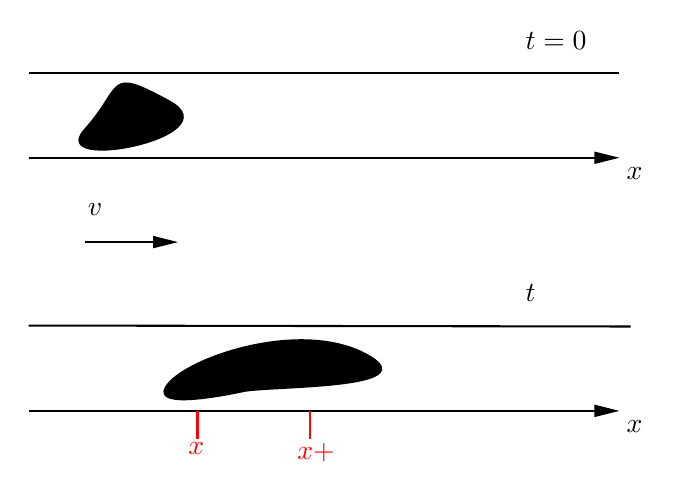
\begin{tikzpicture}[x=0.75pt,y=0.75pt,yscale=-1,xscale=1]
        %uncomment if require: \path (0,242); %set diagram left start at 0, and has height of 242

        %Straight Lines [id:da44049488951792903] 
        \draw    (110,37.1) -- (394.58,37.1) ;
        %Shape: Polygon Curved [id:ds6553683057711202] 
        \draw  [fill={rgb, 255:red, 0; green, 0; blue, 0 } ,fill opacity=1 ] (177.76,50.65) .. controls (208.62,67.37) and (117.98,85.44) .. (137.1,64.21) .. controls (156.23,42.98) and (146.89,33.94) .. (177.76,50.65) -- cycle ;
        %Straight Lines [id:da5485356023961889] 
        \draw    (110,77.76) -- (392.58,77.76) ;
        \draw [shift={(394.58,77.76)}, rotate = 180] [fill={rgb, 255:red, 0; green, 0; blue, 0 }  ][line width=0.08]  [draw opacity=0] (12,-3) -- (0,0) -- (12,3) -- cycle    ;
        %Straight Lines [id:da3109649021932295] 
        \draw    (110,158.61) -- (400,159.07) ;
        %Shape: Polygon Curved [id:ds8713717377881096] 
        \draw  [fill={rgb, 255:red, 0; green, 0; blue, 0 } ,fill opacity=1 ] (272.62,172.62) .. controls (303.48,189.33) and (225.79,187.52) .. (213.19,190.22) .. controls (200.59,192.92) and (166.01,199.22) .. (177.76,186.17) .. controls (189.51,173.12) and (241.75,155.9) .. (272.62,172.62) -- cycle ;
        %Straight Lines [id:da4714509137995375] 
        \draw    (110,199.72) -- (392.58,199.72) ;
        \draw [shift={(394.58,199.72)}, rotate = 180] [fill={rgb, 255:red, 0; green, 0; blue, 0 }  ][line width=0.08]  [draw opacity=0] (12,-3) -- (0,0) -- (12,3) -- cycle    ;
        %Straight Lines [id:da9398787311164047] 
        \draw    (137.1,118.41) -- (179.96,118.41) ;
        \draw [shift={(181.96,118.41)}, rotate = 180] [fill={rgb, 255:red, 0; green, 0; blue, 0 }  ][line width=0.08]  [draw opacity=0] (12,-3) -- (0,0) -- (12,3) -- cycle    ;
        %Straight Lines [id:da8968726381584198] 
        \draw [color={rgb, 255:red, 255; green, 4; blue, 4 } ,draw opacity=1 ]   (191.31,199.72) -- (191.31,213.27) ;
        %Straight Lines [id:da09345282620108719] 
        \draw [color={rgb, 255:red, 255; green, 4; blue, 4 } ,draw opacity=1 ]   (245.51,199.72) -- (245.51,213.27) ;

        % Text Node
        \draw (396.58,81.16) node [anchor=north west][inner sep=0.75pt]  [font=\normalsize]  {$x$};
        % Text Node
        \draw (347.93,15.6) node [anchor=north west][inner sep=0.75pt]  [font=\normalsize]  {$t=0$};
        % Text Node
        \draw (396.58,203.12) node [anchor=north west][inner sep=0.75pt]  [font=\normalsize]  {$x$};
        % Text Node
        \draw (347.93,137.56) node [anchor=north west][inner sep=0.75pt]  [font=\normalsize]  {$t$};
        % Text Node
        \draw (137,98.4) node [anchor=north west][inner sep=0.75pt]  [font=\normalsize]  {${\textstyle v}$};
        % Text Node
        \draw (185.37,213.74) node [anchor=north west][inner sep=0.75pt]  [font=\normalsize,color={rgb, 255:red, 255; green, 0; blue, 0 } ,opacity=1 ]  {$x$};
        % Text Node
        \draw (237.89,213.74) node [anchor=north west][inner sep=0.75pt]  [font=\normalsize,color={rgb, 255:red, 255; green, 0; blue, 0 } ,opacity=1 ]  {$x+\dx$};

    \end{tikzpicture}

\end{figure}
\FloatBarrier

Vogliamo derivare un modello matematico per descrivere l'evoluzione della concentrazione $\displaystyle c=c(x,t)$ della sostanza. Il tasso di variazione della massa che si trova nell'intervallo $\displaystyle [ x,x+\Delta x]$ è dato da
\begin{equation*}
    \frac{\de}{\dt}\int ^{x+\Delta x}_{x} c(y,t) \dy=\int ^{x+\Delta x}_{x} c_{t}(y,t) \dy
\end{equation*}
è pari alla differenza tra il flusso in entrata attraverso $x$ e il flusso in uscita attraverso $x+\dx$. Indicando con $\displaystyle q=q(x,t)$ il flusso di massa che entra nell'intervallo attraverso il punto $x$ al tempo $t$ posso scrivere la conservazione della massa
\begin{equation*}
    \int ^{x+\Delta x}_{x} c_{t}(y,t) \dy=q(x,t) -q(x+\Delta x,t)
\end{equation*}
Dividendo per $\displaystyle \Delta x$ e passando al limite per $\displaystyle \Delta x\rightarrow 0$ si ottiene
\begin{equation}
    c_{t} =-q_{x}
    \label{eq:inquinante-in-canale}
\end{equation}
Ora bisogna decidere con che tipo di flusso di massa abbiamo a che fare o, in altri termini, stabilire una \textbf{legge costitutiva }per $q$:
\begin{itemize}
    \item Per \textbf{convezione} o trasporto, il flusso è determinato dalla sola corrente d'acqua, come se l'inquinante fosse trasportato dal fluido senza espandersi o deformarsi
          \begin{equation*}
              q(x,t) =vc(x,t)
          \end{equation*}
    \item Per \textbf{diffusione}, similmente alla legge di Fourier per il calore, la legge di Fick stabilisce che la diffusione avviene da zone ad alta concentrazione verso zone a bassa concentrazione
          \begin{equation*}
              q(x,t) =-Dc_{x}(x,t)
          \end{equation*}
\end{itemize}

Poiché nel caso dell'inquinante sono presenti sia trasporto che diffusione, sovrapporremo i due effetti:
\begin{equation*}
    q=\text{diffusione} +\text{trasporto} =vc-Dc_{x},\ \ [ q] =MT^{-1}
\end{equation*}
Sostituendo in \eqref{eq:inquinante-in-canale} si trova
\begin{equation*}
    \boxed{c_{t} =Dc_{xx} -vc_{x}}
\end{equation*}
\LezioneS{15/03/2021}

Consideriamo un modello del tipo
\begin{equation}
    u_{t} =Du_{xx} +bu_{x} +cu
    \label{eq:modello-dif-trasp-rea}
\end{equation}
I vari termini rappresentano
\begin{itemize}
    \item $Du_{xx}$, \textbf{diffusione}
    \item $bu_{x}$, \textbf{trasporto} o deriva (drift) con velocità $v=-b$ nella direzione positiva dell'asse $x$
    \item $cu$, \textbf{reazione} ($c >0$, crescita, oppure $c< 0$ decadimento, esponenziale)
\end{itemize}

Qual'è la soluzione fondamentale per \eqref{eq:modello-dif-trasp-rea}, cioè quella soluzione che al tempo iniziale assume distribuzione Dirac in $x=0$? Si può dimostrare che è
\begin{equation}
    \boxed{\Gamma ^{\star }(x,t) =\frac{1}{\sqrt{4\pi Dt}} e^{ct}\exp\left\{-\frac{(x+bt)^{2}}{4Dt}\right\}}
\end{equation}
Se $c=0$ abbiamo la solita $\Gamma $ che si trasporta, se $c\gtrless 0$ la $\Gamma $ viene accentuata o smorzata esponenzialmente.

L'equazione generale in $n$ dimensioni è
\begin{equation*}
    u_{t} = \underbrace{\mathrm{div}(A \nabla u)}_{\text{diffusione}} + \underbrace{\mathrm{div}(\mathbf{b} u) +\mathbf{v} \cdot\nabla u}_{\text{trasporto}} + \underbrace{cu}_{\text{reazione}}
\end{equation*}
dove i termini dipendono in questo modo
\begin{equation*}
    \mathbf{b} =\mathbf{b}(x,t) \ \ \mathbf{v} =\mathbf{v}(x,t) \ \ c=c(x,t)
\end{equation*}
\section{Problema di Cauchy globale \texorpdfstring{$(n=1)$}{n=1}}

Consideriamo il problema di Cauchy globale in $n=1$ dimensioni. La generalizzazione a dimensione $n >1$ è standard, quindi lavoriamo in $n=1$ per semplicità.
\begin{equation*}
    \tag{PCG$_{\text{diffusione,1D}}$}
    \begin{cases}
        u_{t} -Du_{xx} =0 & \text{in} \ \mathbb{R} \times (0,T) \ \ \ \ T\leqslant +\infty \\
        u(x,0) =g(x)      & \text{in} \ \mathbb{R}
    \end{cases}
    \label{eq:pcg-diffusione-1d}
\end{equation*}
dove $g$ è il \textit{dato iniziale} assegnato.

Interpretiamo $u$ come una \textbf{concentrazione di massa, o densità lineare di massa}, nel senso che $u(x,t) \dx$ è la massa che si trova nell'intervallo $(x,x+\dx)$ al tempo $t$.

Sappiamo risolvere \eqref{eq:pcg-diffusione-1d} nel caso di impulso nell'origine $g(x) =\delta (x)$ e di conseguenza anche nel caso di $g(x) =\delta (x-y)$.\footnote{Non è corretto usare l'uguaglianza, intendiamo che le distribuzioni hanno lo stesso effetto tramite il prodotto di dualità.} In questa situazione, la soluzione è data da
\begin{equation*}
    u(x,t) =\Gamma _{D}(x-y,t)
\end{equation*}
È una \textit{unit-source solution}, nel senso che descrive come si evolve una massa unitaria inizialmente concentrata in $y$. Se avessimo una massa totale di $Q$ anziché unitaria avremmo
\begin{equation*}
    u(x,t) =Q\cdotp \Gamma _{D}(x-y,t)
\end{equation*}

\begin{figure}[htpb]
    \centering
    \tikzset{every picture/.style={line width=0.75pt}} %set default line width to 0.75pt        

    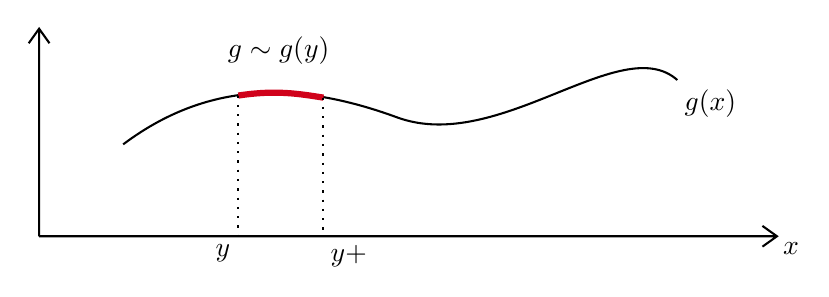
\begin{tikzpicture}[x=0.75pt,y=0.75pt,yscale=-1,xscale=1]
        %uncomment if require: \path (0,140); %set diagram left start at 0, and has height of 140

        %Shape: Axis 2D [id:dp4931078321995175] 
        \draw  (114,110) -- (469.5,110)(114,10) -- (114,110) -- cycle (462.5,105) -- (469.5,110) -- (462.5,115) (109,17) -- (114,10) -- (119,17)  ;
        %Curve Lines [id:da7762158719493701] 
        \draw    (154.5,65.72) .. controls (194.5,35.72) and (237.5,34.72) .. (286.5,52.72) .. controls (335.5,70.72) and (394.5,10.72) .. (421.5,34.72) ;
        %Curve Lines [id:da8187349331902096] 
        \draw [color={rgb, 255:red, 208; green, 2; blue, 27 } ,draw opacity=1 ][line width=2.25]    (210,42.2) .. controls (228.2,39.4) and (239.4,41.4) .. (251,43.2) ;
        %Straight Lines [id:da9080172774216906] 
        \draw  [dash pattern={on 0.84pt off 2.51pt}]  (210,42.2) -- (210,110.4) ;
        %Straight Lines [id:da9068454288868981] 
        \draw  [dash pattern={on 0.84pt off 2.51pt}]  (251,43.2) -- (251,109.4) ;

        % Text Node
        \draw (471,111.4) node [anchor=north west][inner sep=0.75pt]    {$x$};
        % Text Node
        \draw (423.5,38.12) node [anchor=north west][inner sep=0.75pt]    {$g(x)$};
        % Text Node
        \draw (203.5,12.52) node [anchor=north west][inner sep=0.75pt]    {$g\sim g(y)$};
        % Text Node
        \draw (197.5,112.52) node [anchor=north west][inner sep=0.75pt]    {$y$};
        % Text Node
        \draw (253,112.8) node [anchor=north west][inner sep=0.75pt]    {$y+\dx$};

    \end{tikzpicture}

\end{figure}
\FloatBarrier

La massa presente in $(y,y+\dy)$ è $g(y) \dy$. L'evoluzione della singola massa $Q=g(y) \dy$ è
\begin{equation*}
    u(x,t) =\Gamma _{D}(x-y,t) g(y) \dy
\end{equation*}
Per il principio di sovrapposizione possiamo sommare tutti i contributi
\begin{equation*}
    u(x,t) =\int _{\mathbb{R}} \Gamma _{D}(x-y,t) g(y) \dy
\end{equation*}
che è una \textbf{convoluzione} del dato iniziale con la gaussiana
\begin{equation*}
    u(x,t) =(\Gamma _{D}(\cdotp,t) *g)(x)
\end{equation*}
è la \textit{candidata} soluzione di \eqref{eq:pcg-diffusione-1d}.
\subsection{Esistenza}

\textbf{Problemi.}
\begin{enumerate}
    \item L'integrale è ben definito? Se $g(x) \sim e^{|x|^m},m >2$ per $|\x| \rightarrow +\infty $, la gaussiana compensa potenze fino al $2$, quindi ci si aspetta che l'integrale non converga! Non posso scegliere $g$ come voglio, ma dovrò dare delle opportune condizioni all'infinito.
    \item Supponiamo che converga, è vero che $u$ è soluzione dell'equazione differenziale? In altre parole posso passare sotto il segno di integrale?
    \item Supponiamo che sia soluzione, in che senso $u(x,0) =g(x)$?
    \item Se tutto sopra va bene, $u$ è anche l'unica?
\end{enumerate}

Si trova risposta all'esistenza nel seguente fondamentale teorema, dalla dimostrazione piuttosto lunga, che omettiamo.
\begin{theorem}
    [di Esistenza] Sia $g$ una funzione con un numero \textbf{finito} di punti di \textbf{discontinuità} e tale che $\exists c,a$ che la limitano secondo
    \begin{equation}
        \tag{G}
        | g(x)| \leqslant ce^{ax^{2}} \ \ \forall x\in \mathbb{R}
        \label{eq:pcg-diffusione-condizione-g}
    \end{equation}
    Sia
    \begin{equation*}
        u(x,t) =\int _{\mathbb{R}} \Gamma _{D}(x-y,t) g(y) \dy
    \end{equation*}
    Allora
    \begin{enumerate}
        \item $u$ è ben definita e di classe $C^{\infty }$ in ogni strisica del tipo $\mathbb{R} \times (0,T)$, con $T< \frac{1}{4aD}$ e inoltre in tale striscia $u_{t} -Du_{xx} =0$.
        \item Se $x_{0}$ è un punto di continuità per $g$, allora
              \begin{equation*}
                  u(x,t)\rightarrow g(x_{0}) \ \ \text{se} \ (x,t)\rightarrow (x_{0},0)
              \end{equation*}

              In particolare se $g\in C(\mathbb{R})$, allora $u\in C(\mathbb{R} \times [ 0,T])$, \textbf{chiuso} a sinistra.
        \item Esistono due costanti $C,A$ tali che
              \begin{equation*}
                  | u(x,t)| \leqslant Ce^{Ax^{2}} \ \ \forall (x,t) \in \mathbb{R} \times [ 0,T]
              \end{equation*}
    \end{enumerate}
\end{theorem}

Questo risponde a $1,2,3$. Occupiamoci dell'unicità.
\begin{oss}
    In molti casi il dato iniziale $g$ è polinomiale, e il teorema è quindi soddisfatto per ogni scelta di $a$ e $c$, in particolare ci permette di estendere l'invervallo temporale quanto vogliamo essendo $T< \frac{1}{4Da}$, con $a$ arbitrariamente piccolo.
\end{oss}
\begin{oss}
    [Processo regolarizzante] Il primo enunciato sottolinea che anche se il dato iniziale è discontinuo da qualche parte (può esserlo in un numero finito di punti), subito dopo il primo istante la soluzione diventa continua e $C^{\infty }$.
\end{oss}
Per il dato iniziale
\begin{equation*}
    g(x) =\chi _{(-2,0)}(x) +\chi _{(1,4)}(x)
\end{equation*}

\fg{0.7}{diffusione-effetto-regolarizzante}

\begin{oss}
    Se $g$ è limitata (cioè $a=0$ in \eqref{eq:pcg-diffusione-condizione-g}) allora $u$ è definita in $\mathbb{R} \times (0,+\infty)$.
\end{oss}
\subsection{Unicità}

In generale non c'è unicità, vediamo il controesempio di Tychonov. Sia $h$ la funzione definita da:
\begin{equation*}
    h(t) =
    \begin{cases}
        e^{-t^{-2}}, & t >0         \\
        0,           & t\leqslant 0
    \end{cases} \qquad \text{cioè tale che} \ h^{(k)}(t)\xrightarrow{t\rightarrow 0} 0,\ \forall k=0,1,2\dotsc
\end{equation*}
La funzione costruita come
\begin{equation}
    \tag{Tychonov}
    \Tau (x,t) =\sum\limits ^{\infty }_{k=0}\frac{h^{(k)}(t)}{(2k) !} x^{2k}
\end{equation}
è soluzione dell'equazione del calore $\Tau _{t} -\Tau _{xx} =0$ col dato iniziale $\Tau (x,0)=0$ assunto con continuità.
\begin{dimostrazione}
    \ \\
    \begin{enumerate}
        \item[(DE)] Si verifica che
              \begin{equation*}
                  \Tau _{t}(x,t) =\sum\limits _{k=0}^{\infty }\frac{h^{(k+1)}(t)}{(2k) !} x^{2k} =\sum\limits _{k=1}^{\infty }\frac{h^{(k)}(t)}{(2k-2) !} x^{2k-2} =\Tau _{xx}(x,t)
              \end{equation*}
        \item[(IC)] Si dimostra per induzione che $\exists \vartheta  >0$ tale che $\forall t >0$
              \begin{equation*}
                  \left| h^{(k)}(t)\right| \leqslant \frac{k!}{(\vartheta t)^{k}}\exp\left(-\frac{1}{2} t^{-2}\right)
              \end{equation*}possiamo eseguire una maggiorazione
              \begin{align*}
                  | \Tau (x,t)| & =\sum\limits _{k=0}^{\infty }\frac{1}{(2k) !} x^{2k}\left| h^{(k)}(t)\right|                                                                                                     &                                  \\
                                & \leqslant \sum\limits _{k=0}^{\infty }\frac{1}{(2k) !} x^{2k}\frac{k!}{(\vartheta t)^{k}}\exp\left(-\frac{1}{2} t^{-2}\right)                                                    & \text{(usando la maggiorazione)} \\
                                & < \sum\limits _{k=0}^{\infty }\frac{1}{k!} x^{2k}\frac{1}{(\vartheta t)^{k}}\exp\left(-\frac{1}{2} t^{-2}\right)                                                                 & \frac{k!}{(2k) !} < \frac{1}{k!} \\
                                & =\underbrace{\sum\limits _{k=0}^{\infty }\frac{\left(\frac{x^{2}}{\vartheta t}\right)^{k}}{k!}}_{\exp\left(\frac{x^{2}}{\vartheta t}\right)}\exp\left(-\frac{1}{2} t^{-2}\right) &                                  \\
                                & =\exp\left(\frac{x^{2}}{\vartheta t} -\frac{1}{2} t^{-2}\right)                                                                                                                  & \text{(serie esponenziale)}
              \end{align*}

              Per $x$ fissato e $t\rightarrow 0$, allora $| \Tau (x,t)| \rightarrow 0$.
    \end{enumerate}
\end{dimostrazione}
Quindi $\Tau (x,t)$ rispetta l'equazione differenziale e anche il teorema di esistenza. Tuttavia \textbf{anche la soluzione identicamente nulla è, ovviamente, soluzione del problema}. Segue che \textbf{in generale la soluzione non è unica}.

Il problema è che $\Tau $ cresce troppo quando $x\rightarrow \pm \infty $ per tempi $t$ piccoli a causa del termine
\begin{equation*}
    \frac{x^{2}}{\vartheta t}
\end{equation*}
Se al posto di $\vartheta t$ ci fosse una costante andrebbe meglio: si definisce una classe di soluzioni a crescita controllata che garantisce l'unicità.
\begin{definition}
    [Classe di Tychonov]
    \begin{equation*}
        | u(x,t)| \leqslant Ce^{Ax^{2}},\ \ \forall x\in \mathbb{R},t\in [ 0,T]
    \end{equation*}
\end{definition}
\begin{theorem}
    [Principio di massimo globale] Sia $u\in C(\mathbb{R} \times [ 0,T])$, con $u_{t},u_{x},u_{xx}$ continue in $\mathbb{R} \times (0,T)$, tale che in $\mathbb{R} \times (0,T)$
    \begin{enumerate}
        \item Sia una sottosoluzione dell'equazione del calore
              \begin{equation*}
                  u_{t} -Du_{xx} \leqslant 0\ \ \ \ (\geqslant)
              \end{equation*}
        \item Sia dominata da un esponenziale, $C >0$
              \begin{equation*}
                  u(x,t) \leqslant Ce^{Ax^{2}} \ \ \ \ \left(\geqslant -Ce^{Ax^{2}}\right)
              \end{equation*}
    \end{enumerate}
    Allora
    \begin{equation*}
        \sup _{\mathbb{R} \times [ 0,T]} u(x,t) \leqslant \sup _{\mathbb{R}} u(x,0) \qquad \left(\inf_{\mathbb{R} \times [ 0,T]} u(x,t) \geqslant \inf_{\mathbb{R}} u(x,0)\right)
    \end{equation*}
\end{theorem}

Se $u$ fosse soluzione dell'equazione
\begin{equation*}
    \begin{cases}
        u_{t} -Du_{xx} =0                  & \text{in} \ \mathbb{R} \times (0,T) \\
        u\ \text{nella classe di Tychonov} &
    \end{cases}
\end{equation*}
allora
\begin{equation*}
    u(x,0) =0\ \ \text{implica} \ \ u(x,t) =0\ \ \text{in} \ \mathbb{R} \times [ 0,T]
\end{equation*}
\textbf{Conseguenza.}

La
\begin{equation*}
    u(x,t) =\int _{\mathbb{R}} \Gamma _{D}(x-y,t) g(y) \dy
\end{equation*}
definita nel teorema di Esistenza è unica all'interno della Classe di Tychonov, che era comunque richiesta in tale teorema al punto $3$, pertanto fornisce non solo esistenza, ma anche unicità!